\chapter{Solver selection and configuration}
\label{chapter:solver configuration}


\section{Problem statement} \label{subseq:problem-statement}

\todo{from PDEs discretization to ODE}

% from numerical integration to system of linear equations
Numerical integration of time dependent partial differential equations can be achieved using different numerical schemes, namely: Runge-Kutta methods. In numerical analysis, the Runge–Kutta methods are a family of implicit and explicit iterative methods \cite{wiki:runge-kutta}. Implicit and explicit methods have their advantages and disadvantages which can be found in the corresponding literature.\\
% reference on something

 In general, implicit methods are robust in case of stiff equations, however, on another hand they are more expensive in terms of computational cost since they introduce a non-linear part that has to be solve using the Newton's method as an example. There is also a class of integration methods called semi-implicit that were designed to reduce the cost of implicit ones and be able to cope with stiff equations. But in all cases numerical integration boils down to solution of a couple systems of linear equations of a type:


\begin{equation} \label{eq:slq}
	Ax = b
\end{equation}


 where $A \in \mathbb{R^{N \times N}}$ is an invertible square matrix, $b \in \mathbb{R^{N}}$ represents the right-hand side, and $x \in \mathbb{R^{N}}$ is the solution vector. At this point we refer to a system of linear equations as just a system and we will use these two terms interchangeably. \\

 
In some cases, especially in case of implicit or semi-implicit methods, we have to compute several systems to perform one step of numerical integration. Thus, solution of a system \ref{eq:slq} is the computational core of any time integration scheme. In fact, it is the most expensive part and it is primary source of code optimization. \\ 


There are three major ways to solve a system of linear equations, namely: direct dense methods, sparse direct methods and iterative methods.\\

In the following sections \ref{subseq:direct methods}, \ref{subseq:iterative methods}, \ref{subseq:sparse methods} we are briefly going to review all three types of numerical solvers as well as their advantages and disadvantages and some aspects of their parallel implementations with a strong focus on their strong scaling behavior. Strong scaling is important for this research since we want to find a solver and its configuration to solve a certain system with a fixed size as fast as possible. Additionally to that, due to a large number of numerical integration steps, we want to find a robust solver to avoid any application crash during simulations.\\

At this point we can set requirements for a solver that we are looking for:\\

\begin{itemize}
	\item robustness
	\item numerical stability
	\item strong scaling efficiency
	\item open source licenses
\end{itemize}




\section{Matrix sets, hardware, compilers and MPI library} \label{subseq:matrix-sets-and-hardware}

During the stiudy, we we using two matrix sets: GRS and SuiteSparse. In our case, the SiteSparse matrix set was, in fact, few matrices downloaded from SuiteSparse Matrix Collection \cite{sparse-matrix-collection:1}, \cite{sparse-matrix-collection:2}. We tried to choose different matrices from the collection with respect to both the number of equations $n$ in a system and ratio $R$ between the number of non-zero elements $nnz$ and the number of equations.\\ 


\todo{describe what ATHLET is}
To generate GRS matrix set, we ran the most common GRS simulations in ATHLET and stopped the simulations somewhere in the middle saving corresponding shifted Jacobian matrices in the PETSc binary format.\\
\todo{describe what a shifted Jacobian matrix is}

Tables \ref{table:grs-matrix-set}  and \ref{table:suite-sparse-matrix-set} shows matrix properties of both matrix sets.\\


\begin{table}[ht]
\centering
\begin{tabular}{|l|l|l|l|}
\hline
Name     & n       & nnz      & nnz / n \\ \hline
pwr-3d   & 6009    & 117897   & 19.6200 \\ \hline
cube-5   & 9325    & 117897   & 6.0568  \\ \hline
cube-64  & 100657  & 1388993  & 13.7993 \\ \hline
cube-645 & 1000045 & 13906057 & 13.9054 \\ \hline
k3-2     & 130101  & 787997   & 6.0568  \\ \hline
k3-18    & 1155955 & 7204723  & 6.2327  \\ \hline
\end{tabular}
\caption{GRS matrix set}
\label{table:grs-matrix-set}
\end{table}



\begin{table}[ht]
\centering
\begin{tabular}{|l|l|l|l|l|}
\hline
Name        & n       & nnz      & nnz / n & Field                      \\ \hline
cant        & 62451   & 4007383  & 64.1684 & 2D/3D Problem              \\ \hline
consph      & 83334   & 6010480  & 72.1251 & 2D/3D Problem              \\ \hline
CurlCurl\_3 & 1219574 & 13544618 & 11.1060 & Model Reduction Problem    \\ \hline
Geo\_1438   & 1437960 & 63156690 & 43.9210 & 2D/3D Problem              \\ \hline
memchip     & 2707524 & 13343948 & 4.9285  & Circuit Simulation Problem \\ \hline
nlpkkt80    & 1062400 & 28192672 & 26.5368 & Optimization Problem       \\ \hline
PFlow\_742  & 742793  & 37138461 & 49.9984 & 2D/3D Problem              \\ \hline
pkustk10    & 80676   & 4308984  & 53.4110 & Structural Problem         \\ \hline
torso3      & 259156  & 4429042  & 7.0903  & 2D/3D Problem              \\ \hline
x104        & 108384  & 8713602  & 80.3956 & Structural Problem         \\ \hline
\end{tabular}
\caption{SuiteSparse matrix set}
\label{table:suite-sparse-matrix-set}
\end{table}


From now, we are going to introduce and use a definition of \textbf{skinny sparse matrices}. It is matrices with relatively low  ration $R$ i.e. less than 15. \\ 


The objective of this study was to find and configure a solver which could fulfill all requirements listed above for the GRS matrix set. From time to time, we used the SuiteSparse set for comparison reasons. It seems to us that GRS matrix set was different because of some specifics of 1D pipeline discretization. For example, GRS matrices are skinny and blocked, where each block is a small, approximately 3-by-3, dense matrix. Additionally, some rows can contain only one element i.e. on the diagonal. It is a result of dynamic pipeline switching of a reactor cooling system. As we will see in section \ref{subseq:sparse methods}, sparse direct solvers can be quite sensitive to the sparse structure of a matrix.\\


We used different hardware to measure performance of different solvers. The first machine was the GRS cluster (HW1) which was our main target. We used a LRZ CoolMUC-2 Linux cluster (HW2) every time when we got some ambiguous results in order to check whether a problem was hardware or software specific. Table \ref{table:hardware-spec} shows a single node specification of both machines. 


\begin{table}[ht]
\centering
\begin{tabular}{|l|c|c|}
\hline
                    & HW1 (GRS) & HW2 (LRZ Linux) \\ \hline
Architecture        & x86\_64 & x86\_64 \\ \hline
CPU(s)              & 20 &  28 \\ \hline
On-line CPU(s) list & 0-19 &  0-27 \\ \hline
Thread(s) per core  & 1 &  1 \\  \hline
Core(s) per socket  & 10 & 14 \\ \hline
Socket(s)           & 2 &  2 \\ \hline
NUMA node(s)        & 2 &  4 \\ \hline
Model               & 62 &  63 \\ \hline
Model name          & E5-2680 v2 & 
E5-2697 v3 \\ \hline
Stepping            & 4 &  2 \\ \hline
CPU MHz             & 1200.0 &  2036.707 \\ \hline
Virtualization      & VT-x &  VT-x \\ \hline
L1d cache           & 32K &  32K \\ \hline
L1i cache           & 32K &  32K \\ \hline
L2 cache            & 256K &  256K \\ \hline
L3 cache            & 25600K &  17920K \\ \hline
NUMA node0 CPU(s)   & 0-9 &  0-6 \\ \hline
NUMA node1 CPU(s)   & 10-19 &  7-13 \\ \hline
NUMA node2 CPU(s)   & - &  14-20 \\ \hline
NUMA node3 CPU(s)   & - &  21-27 \\ \hline
\end{tabular}
\caption{Hardware specification}
\label{table:hardware-spec}
\end{table}


We decided to stick to the OpenMPI library which is an implementation of the MPI standard. OpenMPI is an open-source project and it is very well documented. The library has many options for processes pinning which was crucial in our study because we had to deal with multi-socket machines which, in turn, had multiple NUMA domains.\\

\textbf{Intel 18.2} compiler was chosen for this study as the newest and the most efficient Intel compiler at the time of writing.\\

\newpage

\section{Direct dense methods} \label{subseq:direct methods}

\todo{MUST BE ONLY 2D Scalapack EXAMPLE HERE}

Direct methods have very good numerical stability properties. They do not require to modify a system of equations as it is necessary for iterative methods. Sometimes we only need to permute some rows and columns in order to avoid small absolute values along the matrix diagonal, which can have their negative effect on numerical accuracy, in case of direct methods. However, this operation can be considered relatively cheap. \\

On another hand, the computational complexity of $O(n^3)$ and storage requirements of $O(n^2)$ make direct methods not suitable for computation of large systems with more than $\sim 10^3$ number of equations. \\


Another good property of direct dense solvers is they have direct memory access and they are based on dense linear algebra subroutines. As a result, implementation of these methods can exploit such programming techniques like cache blocking, tiling, data prefetching,  utilization of hardware vector units and so on. All of these together make it possible to achieve more than 75\% hardware performance of modern CPUs \cite{articles:blas-performance} due to a high ratio of floating point operations per memory access. \\

A general way to solve a system of a type \ref{eq:slq} is to perform $LU$ factorization where a matrix $A$ can be viewed as a product of a lower and upper triangular matrices. 

\begin{equation} \label{eq:lu}
	Ax = LUx = b
\end{equation}

Having computed matrices $L$ and $U$, two additional steps, forward and backward substitutions, are required to compute the solution vector $x$.

\begin{align} \label{eq:bk}
	Ly = b \\
	Ux = y
\end{align}

The main idea of parallel $LU$ decomposition is based on block structure of a matrix $A$. Any given matrix $A$ can be represented as a combination of sub-matrices $A_{ij}$.

$$
A = 
\Bigg(\begin{array}{c|c|c}
A_{11} & A_{12} & A_{13} \\ \hline
A_{21} & A_{22} & A_{23} \\ \hline
A_{31} & A_{32} & A_{33}
\end{array}\Bigg)
$$

This allows to develop algorithms that can compute $LU$ decomposition of the full matrix $A$ in parallel using sub-matrices with three main routines i.e. matrix-matrix multiply, triangular solve with multiple right hand sides and the unblock $LU$ factorization for operation within a block column \cite{netlib:lapack-1}.\\

There exist three well known parallel approaches based on left, right and Crout decomposition forms. All of these three approaches have similar overall performance, with a slight advantage to the right-looking and Crout variants \cite{netlib:lapack-1}. 

% example

Let's consider right-looking algorithm as an example. The algorithm can be written as following:

\begin{equation} \label{eq:RightLookingLu}
\Bigg(\begin{array}{c c}
A_{11} & A_{12} \\
A_{21} & A_{22} \\
\end{array}\Bigg)
=
\Bigg(\begin{array}{c c}
L_{11} & 0 \\
L_{21} & L_{22} \\
\end{array}\Bigg)
\cdot
\Bigg(\begin{array}{c c}
U_{11} & U_{12} \\
0 & U_{22} \\
\end{array}\Bigg)
\end{equation}

The algorithm starts with an assumption that both matrices $L_{11}$ and $U_{11}$ have already been computed. 
% size of the matrix is proportional to the size of the cache

Given equation \ref{eq:RightLookingLu}, we can write expressions for $A_{12}$ and $A_{21}$ matrices:

\begin{align} \label{eq:RightLookingLuFirstUpdate}
A_{12} = L_{11} \cdot U_{12} \\
A_{21} = L_{21} \cdot U_{11}
\end{align}

To compute \ref{eq:RightLookingLuFirstUpdate} we only have to perform two triangular solves since matrices $L_{11}$ and $U_{11}$ are known. These two tasks are concurrent and they can be computed in parallel. Additionally we can notice the triangular solve routine can be computed in parallel too. The next step is to perform $\hat{A_{22}}$ matrix update and block structure re-odering:

\begin{equation} \label{eq:RightLookingLuSecondUpdate}
\hat{A_{22}} = A_{22} - L_{21} \cdot U_{12}
\end{equation}

\figpointer{\ref{fig:RightLookingLuReodering}}
\begin{figure}[htpb]
  \centering
  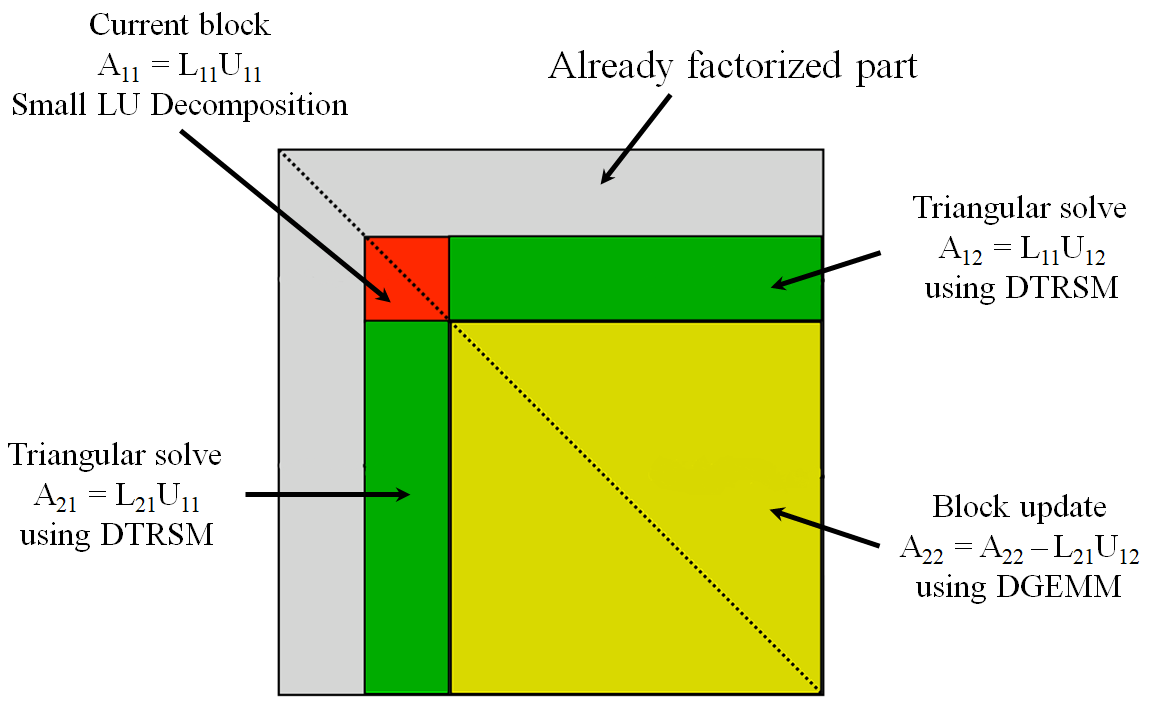
\includegraphics[width=0.75\textwidth]{figures/chapter-2/right-looking-la.png}
\caption{Right-looking parallel LU decomposition}
\label{fig:RightLookingLuReodering}
\end{figure}


% Show limited parallelism
It is clear the algorithm is purely sequential at the first steps when we compute small $LU$ decomposition. Therefore, it can have significant effect on algorithm strong scaling behavior. It should be mentioned that all three parallel implementations have the same problem i.e. they have an inherently sequential part at the beginning of a step. \\

Figure \ref{fig:lapack-lu-strong-scaling} shows results of strong scaling of dense $LU$ factorization performed for a couple of matrices filled with random numbers with different sizes: namely: $5000 \times 5000$, $10000 \times 10000$ and $15000 \times 15000$. LAPACK and OpenBLAS libraries were used for the test. One can easily notice that performance of dense $LU$ decomposition quickly deteriorates with reduction of the problem size. Additional factor that affects performance is strong scaling behavior of the triangular solve that we will discuss in section \ref{subseq:iterative methods}. 

\figpointer{\ref{fig:lapack-lu-strong-scaling}}
\begin{figure}[htpb]
  \centering
  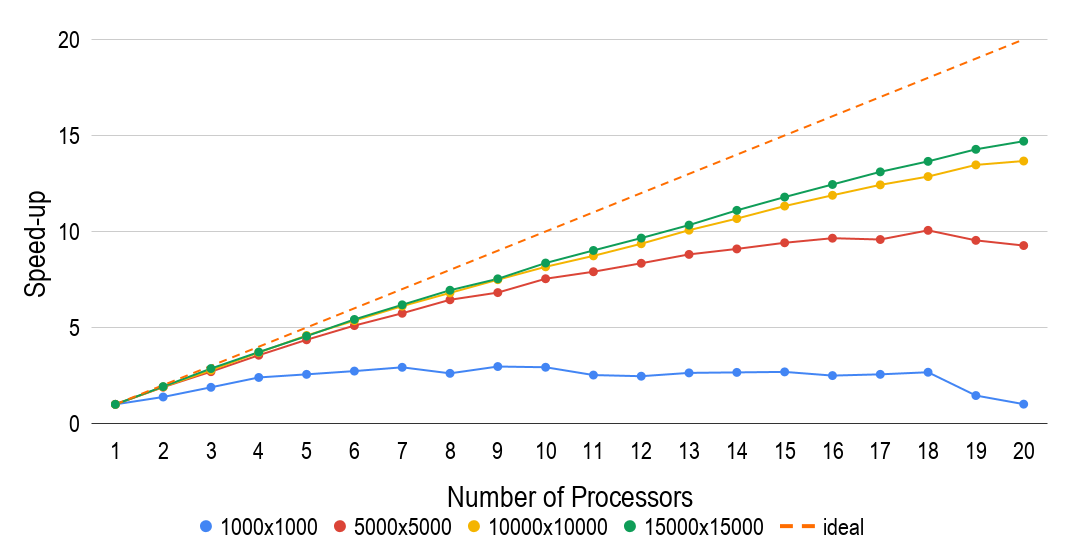
\includegraphics[width=0.85\textwidth]{figures/chapter-2/lapack-lu-strong-scaling.png}
\caption{Strong scaling of right-looking $LU$ decomposition using LAPACK and OpenBLAS}
\label{fig:lapack-lu-strong-scaling}
\end{figure}


\todo{add strong scaling for ScaLAPACK}
% results of strong scaling

Both left, right and Crout parallel matrix factorizations have been efficiently implemented in LAPACK (for shared-memory machines) and ScaLAPACK (distributed-memory machines) libraries. Both libraries belong to the Netlib project which is a repository of numerous scientific computing software maintained by AT\&T Bell Laboratories, the University of Tennessee, Oak Ridge National Laboratory and other scintific communities \cite{netlib-overview}. The libraries are built on top of Basic Linear Algebra Subprograms (BLAS) library. Figure \ref{fig:blas-lapack-scalapack} shows how these three libraries are coupled together.\\


\figpointer{\ref{fig:blas-lapack-scalapack}}
\begin{figure}[htpb]
  \centering
  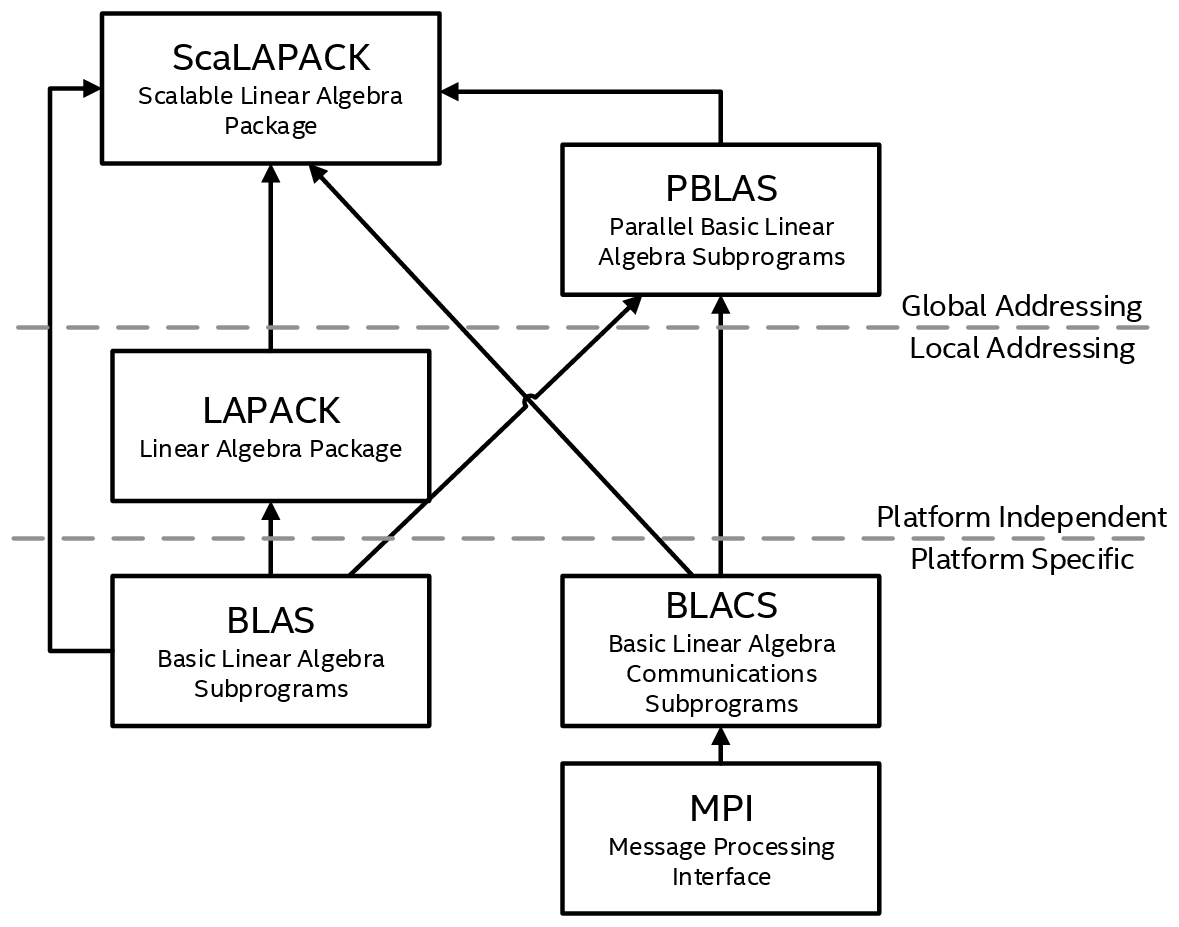
\includegraphics[width=0.65\textwidth]{figures/chapter-2/lapack-scalapack-blas.png}
\caption{A general view on BLAS, LAPACK and ScaLAPACK libraries \cite{netlib:lapack-scalapack-general-view}}
\label{fig:blas-lapack-scalapack}
\end{figure}

It is worth noting that BLAS can be considered as a foundation of LAPACK and ScaLAPACK libraries and, thus, it is the primary source of performance improvement. In particular we have to consider DGEMM, DTRSM BLAS subroutines performance because they, together with unblocked $LU$ factorization, compose the core of parallel $LU$ factorization algorithms as we discussed earlier.\\

There exist special-purpose, hardware-specific BLAS implementations developed by the hardware vendors i.e. IBM, Cray, Intel, AMD as well as open-source tuned implementations such as ATLAS, OpenBLAS, etc. We will come back to that discussion later and pay our close attention to a specific choice of a tuned BLAS library in subsection \ref{subseq:blas-comparison}.\\

In spite of all advantages of the direct dense solvers i.e. numerical stability and high ratio of floating point operations per memory access, we cannot consider this group of methods as a solver for time integration due to high complexity and storage costs.


\section{Iterative methods}
\label{subseq:iterative methods}
Iterative methods, especially Krylov subspace methods that we are going to discuss in this section, are well known for their relatively low storage requirements $O(nnz)$ and computation cost $O(N^2)$ in case of sparse linear systems of equations and good condition number. It turns out that sometimes it might be only one way to solve huge systems with millions unknowns.\\

The most well known methods are Conjugate Gradient (CG) for symmetric positive definite matrices, Minimal Residual Method (MINRES) for symmetric indefinite systems, Generalized Minimal Residual Method (GMRES) for non-symmetric systems of linear equations as well as different variants of GMRES such Biconjugate Gradient Method (BiCG), Biconjugate Gradient Stabilized Method (BiCGSTAB) and so on.\\

All Krylov methods solve a system of equation as a minimization problem. For example, the goal of CG algorithm is to minimize the energy functional $f(x) = 0.5 x^T A x - b^T x + c$, whereas, MINRES and GMRES tries to minimize residual norm $r_{j}$ for $x_{j}$ in a subspace. \\

%$j$th Krylov subspace $\mathcal{K}_{j}$. \\

The methods construct an approximate solution of a system as a linear combination of vectors $b$, $Ab$, $A^2b$, $A^3b$ and so on which defines the Krylov subspace. At each iteration we expand the subspace adding and evaluating a next vector in the combination.\\

Let's consider GMRES, as the most popular and general iterative solver, without preconditioning to just analyze its strong scaling behavior and potential problems. \\ 

As we mentioned above GMRES minimizes the residual norm in a subspace $U_m$.

\begin{equation} \label{eq:Gmres-1}
	\underset{x \in U_m}{min}||Ax - b||^2
\end{equation}

We can consider a solution vector $x$ in the subspace $U_m$ in a form $x=U_m y$. Thus, equation \ref{eq:Gmres-1} can be written as following:

\begin{equation} \label{eq:Gmres-2}
	\underset{x \in U_m}{min}||AU_m y - b||^2
\end{equation}

The most natural way to choose a proper subspace $U_m$ is the corresponding Krylov subspace $\mathcal{K}_m$ because it can be easily generated on the fly. However, decomposition of vector $x$ in that subspace can be a problem. Since the subspace $\mathcal{K}_m$ is spanned by the sequence of $b$, $Ab$, $A^2b$, ..., $A^{m-1}b$ and due to round-off error the sequence can become linear dependent. Therefore, we have to compute and use the orthonormal base of the given Krylov subspace. Saad and Schultz in their work \cite{sparse-la:gmrese-origin} used Arnoldi process for constructing an $l_2$-orthogonal basis. As the results equation \ref{eq:Gmres-2} can be written in the following form:  \\

\begin{equation} \label{eq:Gmres-3}
	\underset{x \in U_m}{min}||U_{m+1}H_{m+1,m} y - ||b||u_1||^2 = \\
	\underset{x \in U_m}{min}||H_{m+1,m} y - ||b||e_1||^2 
\end{equation}

where $H_m$ is an upper Hessenberg matrix. We can apply Givens rotation algorithm to compute $QR$ decomposition to convert $H_m$ to a strictly upper triangular matrix. Thus,

 
\begin{equation} \label{eq:Gmres-4}
	\underset{x \in K_m}{min}||Ax - b||^2 = \\
	\underset{x \in U_m}{min}||Q^TRy - ||b||e_1||^2 = \\
	\underset{x \in U_m}{min}||\Big(\begin{array}{c c}R_m \\ 0 \\\end{array}\Big) y - \Big(\begin{array}{c c} \tilde{b_m} \\ \tilde{b_{n-m}} \\\end{array}\Big)||^2
\end{equation}

Given \ref{eq:Gmres-4}, we can compute the solution as following:

\begin{equation} \label{eq:Gmres-5}
	R_m y = \tilde{b_m}
\end{equation}


\begin{equation} \label{eq:Gmres-6}
	x_m = U_m y  
\end{equation}

Because of large computational and storage costs, in case of evaluation of the full Krylov subspace, only small a subspace is computed, typically first 20 - 50 column vectors. Then the algorithm is restarted using the computed approximate solution as a initial guess for the next iteration.\\

We can see that some operations, for example \ref{eq:Gmres-6}, can be efficiently done in parallel. However, operatiopns like sparse triangular solve \ref{eq:Gmres-5} can introduce some effect on strong scaling behavior. Figure \ref{fig:sparse-triangular-solve-performance} shows strong scaling performance results of a sparse parallel triangular solver with a two dimensional matrix distribution. Performance considerations of the solver can be found in \cite{sparse-la:triangular-solve}.\\

\figpointer{\ref{fig:sparse-triangular-solve-performance}}

\begin{figure}[htpb]
  \centering
  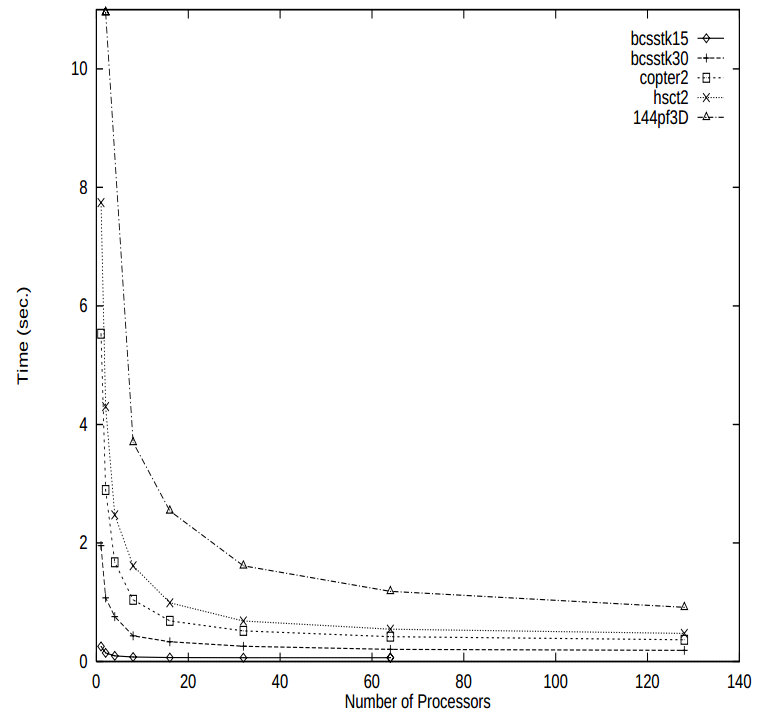
\includegraphics[width=0.5\textwidth]{figures/chapter-2/sparse-triangular-solve-performance.png}
\caption{Performance of sparse triangular solve \cite{sparse-la:triangular-solve}}
\label{fig:sparse-triangular-solve-performance}
\end{figure}


It is interesting to notice that performance of the triangular solver depends on a matrix sparsity structure as well as the matrix size. \\

Triangular solve \ref{eq:Gmres-5} can be computed in a single processor because matrix $R_m$ is usually small and depends on the number iterations before the restart. In this case the triangular solve can become a bottleneck again. \\

Figure \ref{fig:gmres-strong-scaling-speed-up} shows strong scaling performance results of the default GMRES solver from the PETSc library. The solver was set up without any preconditioner and 50 iterations as the restart. Additionally no stop criteria was specified except the maximum number iterations which was equal to 100. Four different matrices with different sparsity patterns were examined for the test. The information about the matrices is summarized in table \ref{table:matrix-info-1}. As we expected we can observe strong deviation of our test cases from the ideal speed-up when the number of processes exceeds 10.\\

It should be mentioned that parallelization overheads, introduced by such MPI operations as MPI\_Send, MPI\_Recv, MPI\_Allreduce, etc., also have their impact on performance of the algorithm.\\

\begin{table}[htpb]
\centering
\begin{tabular}{|c|c|c|c|}
\hline
Matrix Name & n       & nnz      & nnz / n \\ \hline
k3-18       & 1155955 & 7204723  & 6.2327  \\ \hline
k3-2        & 130101  & 13906057 & 6.0568  \\ \hline
cube-645    & 1000045 & 787997   & 13.9054 \\ \hline
cube-64     & 100657  & 1388993  & 13.7992 \\ \hline
\end{tabular}
\caption{Basic information about matrices used in figure \ref{fig:gmres-strong-scaling-speed-up}}
\label{table:matrix-info-1}
\end{table}

Other Krylov methods such as CG, for example, scales much better than GMRES. Because of the nature of the CG algorithm the next search direction can be found using a recurrent expression and the algorithms boils down to simple operations such as dot products and matrix vector multiplications. These operations can be easily parallelized and drop of performance comes only from MPI overheads. A quite comprehensive study about parallel CG algorithm performance can be found in \cite{sparse-la:cg}. The authors also introduced a deeply pipelined version of CG algorithm that scales even better due to overlapping the time-consuming global communication phase, induced by parallel dot product computations, with useful independent computations \cite{sparse-la:cg}.\\


\figpointer{\ref{fig:gmres-strong-scaling-speed-up}}
\begin{figure}[htpb]
  \centering
  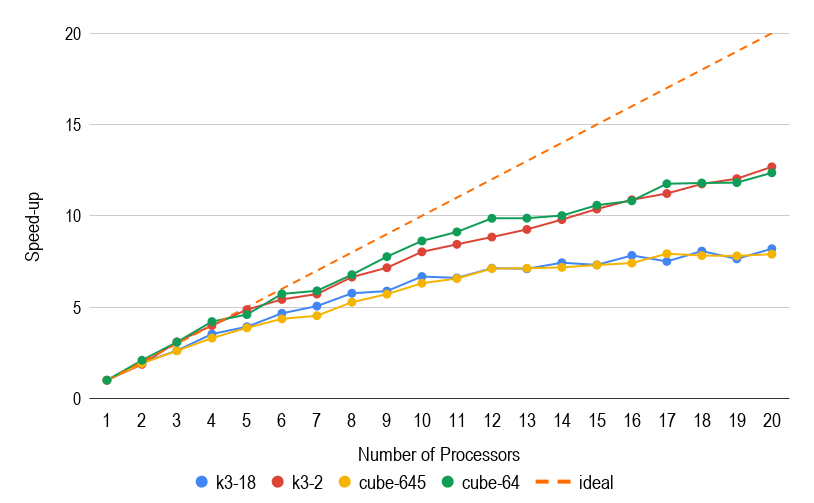
\includegraphics[width=0.8\textwidth]{figures/chapter-2/gmres-strong-scaling-speedup.png}
\caption{GMRES strong scaling speed-up}
\label{fig:gmres-strong-scaling-speed-up}
\end{figure}



% start discussion about preconditioning
The most important criteria of Krylov methods is convergence rate. The convergence rate of iterative methods strongly depends on a matrix and, in particular, on its condition number. For instance, equation \ref{eq:Gmres-7} shows dependence of the convergence rate from the matrix condition number. It can be clearly seen that a big condition number leads to very slow error reduction and, as the results, to huge number of iterations.\\

\begin{equation} \label{eq:Gmres-7}
	|| e^i ||_A \leq 2 ( \frac{\sqrt k - 1}{\sqrt k + 1} )^i || e^0 ||_A
\end{equation}

where $k = \frac{\lambda_{max}}{\lambda_{min}}$ - condition number of the corresponding matrix. \\

An obvious solution of such a problem is to reduce the condition number of the original system \ref{eq:slq}. A general method is to transform the original system in such a way that the conditional number of the transformed system gets significantly smaller. The transformation of \ref{eq:slq} can be done from the left side \ref{eq:pcn-1} or from the right one \ref{eq:pcn-2}.

\begin{equation} \label{eq:pcn-1}
	PAx = Pb
\end{equation}


\begin{equation} \label{eq:pcn-2}
	AP(P^{-1}x) = b
\end{equation}

where matrix $P$ is called preconditioner.\\


As an extreme example we can consider the inverse matrix $A^{-1}$ as the best preconditioner since it directly leads to the solution of the problem \ref{eq:slq} and, thus, it requires only one iteration. However, it is obvious that computation of inverse $A^{-1}$ is extremely expensive operation and it is not an objective of any iterative methods. That example helps understand and set requirements for preconditioners, namely:

\begin{enumerate}
	\item cheap to compute e.g. a 5-10 iterations of the corresponding Krylov solver
	\item should lead to a small conditioner number of the transposed system
	\item should be sparse, otherwise storage requirements will considerably increase
\end{enumerate}


There exist numerous techniques to compute preconditioners given a matrix $A$ e.g. (point) Jacobi, Block-Jacobi, incomplete $LU$ decomposition (ILU), multilevel ILU (ILU(p)), threshold ILU (ILUT), incomplete Cholesky factorization (IC), sparse approximate inverse (SPAI), multigrid as a preconditioner, etc. Almost all methods listed above have some tuning parameters which allow to get a better preconditioner i.e. a smaller condition number of the transformed system. However, it usually leads to increase of computational and storage costs. \\

Some methods can works particularly well for matrices derived from certain PDEs e.g. Poisson, Navier\-Stokes, etc. problems discretized using the cartesian grid. However sometimes it can take a considerable amount of time to choice right parameters for a certain preconditioning algorithm. It can become a challenge to fulfill all requirements 1, 2, 3 mentioned above. \\

Table \todo{Table with comparisons of different preconditioning for our test cases}

Table [] shows results of different preconditioning algorithms application to our test case. It can be seen that some algorithms failed even after tuning. \\

It interesting to notice that \citeauthor{wsmp} came to approximately the same results working on their set of matrices in their work \cite{wsmp}. They observed that preconditioned iterative solvers worked efficiently only for 2 out 5 cases in contrast to direct sparse solvers.\\

We can summarize that it is vital to perform careful parameter tuning of any preconditioning algorithms combining results from [table] and \cite{wsmp}. In general the  search can take a considerable amount of time. Moreover, it becomes impractical for time integration problems where topology of an underlying problem and, as the results, the computational mesh, discretization, Jacobian matrix can be changed over time of a simulation. It is obvious that parameters chosen for a particular time step can become not optimal for consecutive steps and, at the end, it can lead to divergence. If divergence happens at any time step the entire time integration algorithm fails and the simulation has to be restarted with different preconditioning parameters or with a different preconditioning algorithm.\\

By and large we come to a conclusion that preconditioned iterative solvers are not robust and thus cannot fully fulfill requirements listed in section \ref{chapter:solver configuration}.\\

% maybe above we have to mention inderect memory access and its effect on performance


\section{Direct sparse methods}
\label{subseq:sparse methods}

Direct sparse methods combine main advantages of direct and iterative methods i.e. numerical robustness and usage of sparsity structures. As a results, there is no need for preconditioning and the computation complexity is $O(n^2)$ \cite{complexity-of-spdm}. The problem is that storage cost can significantly increase during factorization i.e. the inverse of a sparse matrix can be sufficiently dense. To reduce storage space of $LU$ decomposition this group of methods performs fill-in reduction reodering as a pre-processing step before actual factorization. If storage space is still huge even after fill-in reduction reodering out-of core factorization can be used where partial results are stored in the secondary memory. \\

The most widely known sparse direct method is multifrontal method introduced by \citeauthor{mult-frontal-original:1} in their work \cite{mult-frontal-original:1}. Multifrontal method is an improved extension of a frontal method \cite{frontal-original} that can compute independent fronts in parallel. A front, or also called frontal matrix, can be considered as small dense matrix which is a result of Gaussian Elimination for a particular column. The algorithm, in fact, is as a variant of Gaussian Elimination process. There also exist left-looking and right-looking sparse direct methods. The difference between all of them is explained and can be found in \cite{elimination-tree}.\\


In order to understand and analyze strong scaling behavior of the algorithm we have to briefly discuss the theory of the method. For simplicity we will assume that matrix $A$ is real symmetric and $LU$ decomposition boils down to the Cholesky factorization \ref{eq:chol-1}. It allows us to focus on the Cholesky factor $L$ and its sparsity pattern only.

\begin{equation} \label{eq:chol-1}
	A = LDL^T
\end{equation}

The algorithm usually starts with symbolic factorization to predict sparsity pattern of $L$. Once it is done the corresponding elimination tree has to be constructed.\\

\figpointer{\ref{fig:sparsity-pattern-example-mm}}

\begin{figure}[htpb]
  \centering
  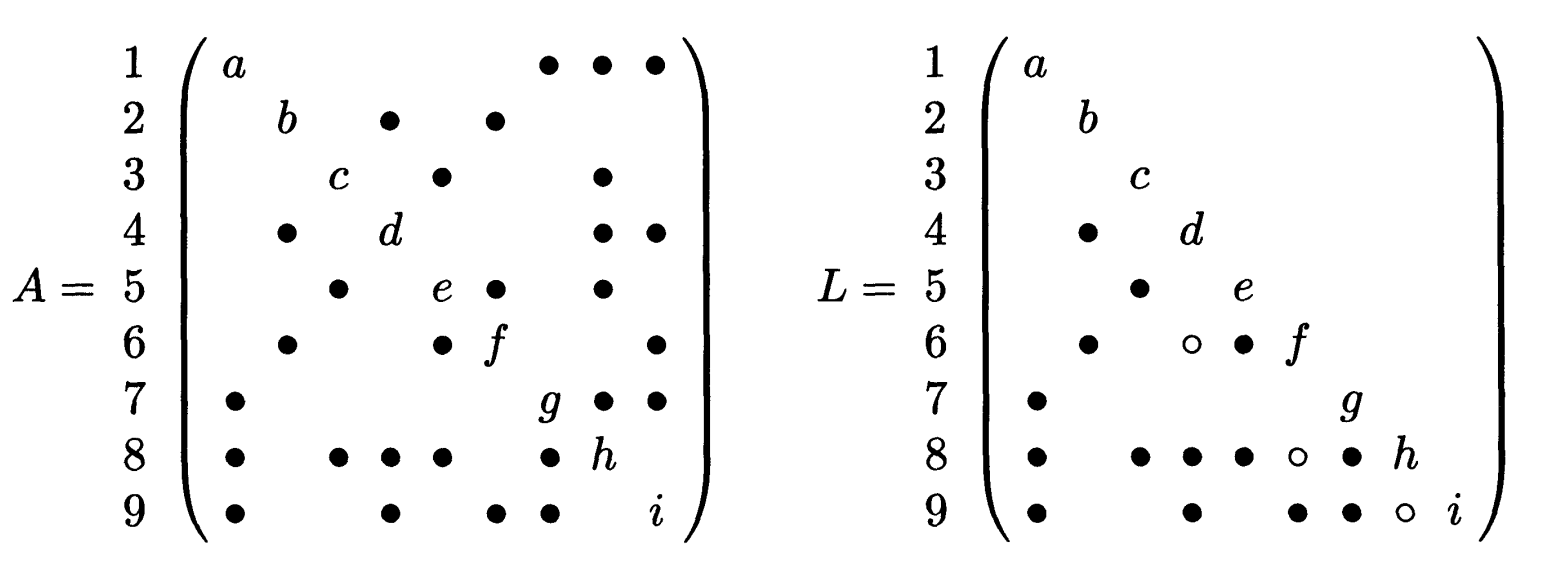
\includegraphics[width=0.9\textwidth]{figures/chapter-2/sparsity-pattern-example-mm.png}
\caption{An example of a sparse matrix and its Cholesky factor \cite{mult-frontal-original:2}}
\label{fig:sparsity-pattern-example-mm}
\end{figure}


Figure \ref{fig:sparsity-pattern-example-mm} shows an illustrative example of a sparse matrix and its Cholesky factor from \cite{mult-frontal-original:2}. The solid circles represent original non-zero elements whereas hollow ones define fill-in factors of $L$. \\


The elimination tree is a crucial part of the method. It can be considered as a structure of $n$ nodes that node $p$ is the parent of $j$ if and only if it satisfies equation \ref{eq:elimination-tree-1}. It is worth pointing out the definition \ref{eq:elimination-tree-1} is not only one possible and one can define a strucutre of an elimination tree in a different way as well. As an example one can find a definition of a general assembly tree in \cite{mult-frontal-original:2} proposed by \citeauthor{mult-frontal-original:2}.\\

\begin{equation} \label{eq:elimination-tree-1}
	p = min(i > j | l_{ij} \neq 0)
\end{equation}


It is important to notice that node $p$ represents elimination process of the corresponding column $p$ of matrix $A$ as well as all dependencies of column $p$ factorization on the results of its descendants.\\


Given definition \ref{eq:elimination-tree-1} we can build the corresponding elimination tree as it is shown in figure \ref{fig:elimination-tree-mm}.\\


\figpointer{\ref{fig:elimination-tree-mm}}

\begin{figure}[htpb]
  \centering
  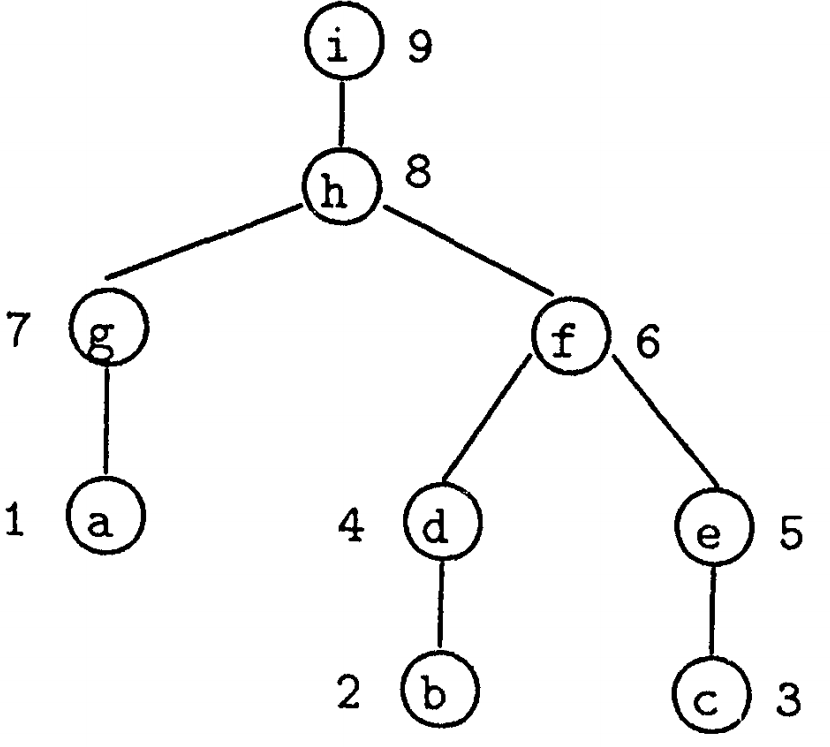
\includegraphics[width=0.45\textwidth]{figures/chapter-2/elimination-tree-mm.png}
\caption{The elimination tree for the matrix example in Figure \ref{fig:sparsity-pattern-example-mm}
 \cite{mult-frontal-original:2}}
\label{fig:elimination-tree-mm}
\end{figure}


The fundamental idea of multifrontal method spins around frontal and update matrices. A frontal matrix is used to perform Gaussian Elimination for a specific column $j$. It is a sum of a frame and update matrices as it can be seen from equation \ref{eq:mm-1}\\.

\begin{equation} \label{eq:mm-1}
	F_{j} = Fr_{j} + \hat{U_{j}} = \begin{bmatrix}a_{j,j} & a_{j,i_1} & a_{j,i_2} & \dots & a_{j,i_r} \\
a_{i_1,j} \\
a_{i_1,j} \\
\vdots & & & 0\\
a_{i_r,j} \\
\end{bmatrix} + \hat{U_{j}}
\end{equation}

where $i_{0}$, $i_{1}$, \dots , $i_{r}$ are the row subscripts of non-zeros in $L_{*j}$ with $i_{0} = j$ and $r$ is number of off-diagonal non-zero elements.\\

The frame matrix $Fr_{j}$ is filed with zeros except the first row and column. The first row and column contain non-zeros elements of the $j$th row and column of the original matrix $A$. Because we consider matrix $A$ to be symmetric the frame matrix is square and symmetric as well.\\

In order to describe parts of the elimination tree we will use the notation $T[j]$ to represent all descendants of the node $j$ in the tree and node $j$ itself. In this way we can define the update matrix $\hat{U_{j}}$ as following:\\

\begin{equation} \label{eq:mm-2}
	\hat{U_{j}} = - \sum_{k \in T[j] -{j}}  \begin{bmatrix}
l_{j,k} \\
l_{i_1,k} \\
\vdots \\
l_{i_1,k} \\
\end{bmatrix} \begin{bmatrix}
l_{j,k} & l_{i_1,k} & \dots & l_{i_1,k}
\end{bmatrix} 
\end{equation}


The update matrix $\hat{U_{j}}$ is, in fact, can be considered as the second term of the Schur complement i.e. update contributions from already factorized columns of $A$.\\

The subscript $k$ represents descendant columns of node $j$. Thus we include and consider only those elements of descendant columns which correspond to the non-zero pattern of the $j$th column that we are currently factorizing.\\

Let's consider the partial factorization of 2-by-2 block dense matrix to better understand essence of update matrix $\hat{U_{j}}$.\\


\begin{equation} \label{eq:mm-3}
A = \begin{bmatrix}
B & V^{T} \\
V & C
\end{bmatrix} 
= 
\begin{bmatrix}
L_{B} & 0 \\
VL^{-T}_{B} & I
\end{bmatrix}
\begin{bmatrix}
I & 0 \\
0 & C - VB^{-1}V^{T}
\end{bmatrix} 
\begin{bmatrix}
L^{T}_{B} & L^{-1}_{B}V^{T} \\
0 & I
\end{bmatrix} 
\end{equation}

Again we assume that $B$ has already been factorized and can be expressed as:

\begin{equation} \label{eq:mm-4}
	B = L_{B}L^{T}_{B}
\end{equation}

The Schur complement from equation \ref{eq:mm-3} can be viewed as the original sub-matrix $C$ and update $-VB^{-1}V^{T}$. It can be written in a vector form as well:

\begin{equation} \label{eq:mm-5}
	-VB^{-1}V^{T} = -(VL^{-T}_{B})(L^{-1}_{B}V^{T}) = - \sum_{k=1}^{j-1}  \begin{bmatrix}
l_{j,k} \\
\vdots \\
l_{n,k} \\
\end{bmatrix} \begin{bmatrix}
l_{j,k} & \dots & l_{n,k}
\end{bmatrix} 
\end{equation}

As it can be easily seen that equations \ref{eq:mm-5} and \ref{eq:mm-2} are identical. The difference is that equation \ref{eq:mm-2} exploits sparsity of the corresponding row and column of $L$ and thus masks unnecessary information. \\

% both eqautions show that the update matrix aggregate all previous information done and in case of the ,ultifrontal methods it means that we aggregate all information from descendants

% Therefore, we can express Uy as an aggregate of outer- product updates from columns in T[Cl],..., T[cs]. 

We can also notice from equation \ref{eq:mm-3} that the frame matrix $Fr_{j}$ corresponds to the block matrix $C$ and brings information from the original matrix $A$ whereas matrix $\hat{U_{j}}$ adds information about the columns that have already been factorized.\\

As soon as the frontal matrix $F_{j}$ is assembled i.e. we have the complete update of column $j$, we can perform elimination of the first column and get non-zero entries of factor column $L_{*j}$.\\

Let's denote $\hat{F_{j}}$ as a result of the first column factorization of the frontal matrix $F_{j}$. Then we can express the results as following:\\


\begin{equation} \label{eq:mm-6}
\hat{F_{j}} = \begin{bmatrix}
l_{j,j} & \dots & 0 \\
\vdots & I \\
l_{i_{r},j} \\
\end{bmatrix} 
\begin{bmatrix}
1 & \dots & 0 \\
\vdots & U_{j} \\
0 \\
\end{bmatrix} 
\begin{bmatrix}
l_{j,j} & \dots & l_{i_{r},j} \\
\vdots & I \\
0 \\
\end{bmatrix} 
\end{equation}

where sub-matrix $U_{j}$ represents the full update from all descendants of node $j$ and node $j$ itself. Equation \ref{eq:mm-7} express the sub-matrix $U_{j}$ in a vector form.\\

\begin{equation} \label{eq:mm-7}
\hat{U_{j}} = - \sum_{k \in T[j]}  \begin{bmatrix}
l_{i_1,k} \\
\vdots \\
l_{i_1,k} \\
\end{bmatrix} \begin{bmatrix}
l_{i_1,k} & \dots & l_{i_1,k}
\end{bmatrix}
\end{equation}

Together with the frontal $F_{j}$ and update $\hat{U_j}$ matrices, the update column matrix $U_{j}$ (also called contribution matrices) forms the key concepts of the multifrontal method. To consider the importance of sub-matrix $U_{j}$ let's consider and example illustrated in Figure \ref{fig:information-float}.\\

\figpointer{\ref{fig:information-float}}
\begin{figure}[htpb]
  \centering
  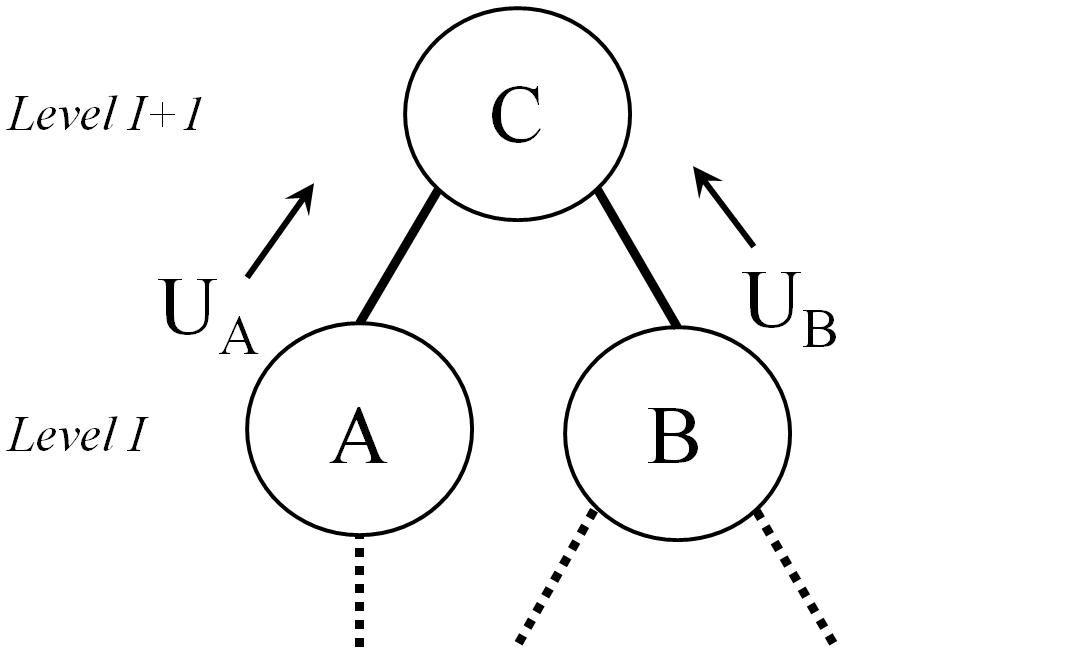
\includegraphics[width=0.45\textwidth]{figures/chapter-2/information-flow.png}
\caption{Information flow of the multifrontal method}
\label{fig:information-float}
\end{figure}


We assume that factorization of columns A and B have already been done and corresponding contribution matrices $U_{A}$ and $U_{B}$ have been computed. From equation \ref{eq:mm-7} we have already known that both $U_{A}$ and $U_{B}$ contain the full updates of all their descendants including updates from factorization of columns $A$ and $B$ as well. Therefore update column matrices $U_{A}$ and $U_{B}$ have already got all necessary information to construct update matrix $\hat{U_{C}}$. The detailed proof and careful explanation can be found in \cite{mult-frontal-original:2}.\\


It might happen that we do not need all rows and columns of $U_{A}$ and $U_{B}$ i.e. we need only some subset of them, because of sparsity of column $C$ . It is also important to place all necessary rows and columns of matrices $U_{A}$ and $U_{B}$ in a right place within matrix $\hat{U_{C}}$. For that reason, an additional matrix operation, called \textbf{\textit{extend-add}}, must be introduced.\\

Let's consider an example from \cite{mult-frontal-original:2} of an extend-add operation for 2-by-2 matrices $R$ and $S$ which correspond to the indices ${5,8}$ and ${5,9}$ of some matrix $B$, respectively.\\

\begin{equation}
R = \begin{bmatrix}
p & q \\
u & v \\
\end{bmatrix} 
,
\:
S = \begin{bmatrix}
w & x \\
y & z \\
\end{bmatrix} 
\end{equation}

The result of the operation is going to be a 3-by-3 $K$ matrix which looks as following:\\

\begin{equation} \label{eq:mm-8}
K = R \extendadd S = \begin{bmatrix}
p & q & 0 \\
u & v & 0 \\
0 & 0 & 0 \\
\end{bmatrix} 
+
\begin{bmatrix}
w & 0 & x \\
0 & 0 & 0 \\
y & 0 & z \\
\end{bmatrix} 
=
\begin{bmatrix}
p + w & q & x \\
u & v & 0 \\
y & 0 & z \\
\end{bmatrix} 
\end{equation}

Hence we can express formation of the frontal matrix $F_{j}$ using the extend-add operation and all direct children of node $j$ in the following way:


\begin{equation} \label{eq:mm-9}
	F_{j} = \begin{bmatrix}a_{j,j} & a_{j,i_1} & a_{j,i_2} & \dots & a_{j,i_r} \\
a_{i_1,j} \\
a_{i_1,j} \\
\vdots & & & 0\\
a_{i_r,j} \\
\end{bmatrix} \extendadd U_{c_1} \extendadd \dots \extendadd U_{c_s} 
\end{equation}

where $c_{1}, \: c_{2}, \: \dots \: c_{n}$ are indices of direct children of the node $j$.\\

Now it can be clearly seen that the resultant frontal matrix $F_{j}$ is a small dense one and it can be efficiently computed using BLAS level 3 subroutines.\\

After factorization we have to build the contribution matrix $U_{j}$ i.e. add columns and rows of $U_{c_1}, \:, U_{c_2}, \: \dots, U_{c_s}$ to $U_{j}$ that have not been used in factorization of $F_{j}$ due to sparsity of column $j$. After that we can continue to move up along the tree. 
The complete update matrices grow in size as we move to the top of the tree. Therefore they have to be stored in a sparse matrix format to stay within memory constrains of the computer.\\


Another important aspect is storage and manipulation of frontal and contribution matrices. Sometimes we have to store contribution matrices produced in previous steps into some temporary buffer and efficiently retrieve them later during factorization. This can require some matrix re-ordering. In case of symmetric matrices, one can apply postordering on a tree to be able to use the stack data structure to alleviate the process of contribution matrix manipulations during factorization. A tree postordering is based on topological ordering and it has been proven that it is equivalent to the original matrix ordering and thus leads to the same filled graph \cite{mult-frontal-original:2}. \todo{sentence refactoring} We refer to the original matrix ordering as the ordering received from fill-in reduction operation.\\


A tree postordering means that a node is ordered before its parent and, additionally, nodes in each subtree are numbered consecutively. Figure \ref{fig:mm-matrix-postordering} shows an example of posrordering applied to the elimination tree of the matrix from figure \ref{fig:sparsity-pattern-example-mm}. The results of this can be see in figure \ref{fig:mm-contrib-matrix-manipulation} where consecutive \textit{push} and \textit{pop} operations are efficiently used during factorization and thus simplify the program logic.\\


\figpointer{\ref{fig:mm-matrix-postordering}}
\begin{figure}[htpb]
  \centering
  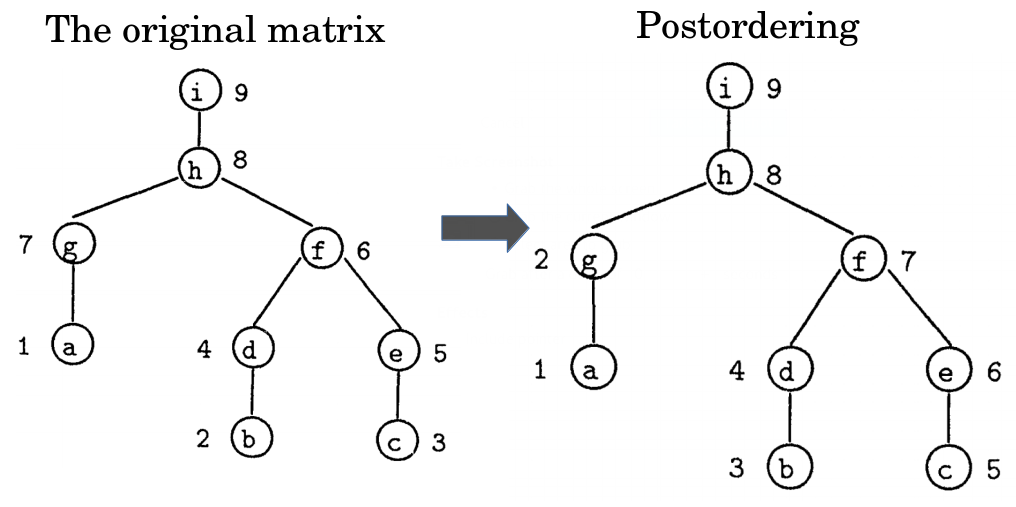
\includegraphics[width=0.75\textwidth]{figures/chapter-2/elimination-tree-mm-postordering.png}
\caption{An example of matrix postordering from \cite{mult-frontal-original:2}}
\label{fig:mm-matrix-postordering}
\end{figure}


\figpointer{\ref{fig:mm-contrib-matrix-manipulation}}
\begin{figure}[htpb]
  \centering
  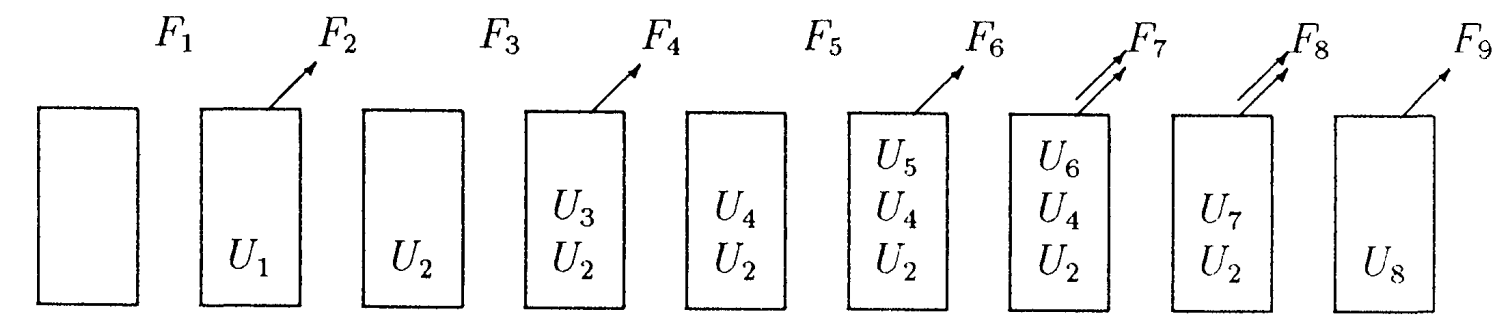
\includegraphics[width=0.75\textwidth]{figures/chapter-2/mm-contrib-matrix-manipulation.png}
\caption{The stack contents for the postordering \cite{mult-frontal-original:2}}
\label{fig:mm-contrib-matrix-manipulation}
\end{figure}


We can see the algorithm requires to perform some preprocessing steps in order to estimate the size of working space for matrix manipulations. If the working space has not been predicted correctly the algorithm will terminate during factorization. Additionally it can happen that even with the correct estimation we can be run out of space in the main memory, in case of huge sparse matrices. This fact can require to use the secondary memory and, as a result, the execution time will increase significantly. Therefore, different optimal postordering schemes have been proposed which allow to shrink the amount of space needed during factorization \cite{mm:optimal-tree-postordering} \cite{mm:elimination-tree-rotations}. Some schemes, for example elimination tree rotations \cite{mm:elimination-tree-rotations}, can lead to deep and unbalanced trees which might have their negative effect on task parallelism as we will see later.\\


In general, the estimation of working space can be tricky due to pivoting. Because pivoting happens only during the numerical factorization it is not always possible to estimate enough space correctly beforehand. There exist some heuristics which allow to use some numerical matrix information during symbolic factorization to better predict the amount of required space \cite{wsmp:direct-solution-of-general-system}.\\



It can be clearly observed the method consists of three distinct phases, namely: analysis, numerical factorization and solution. The analysis phase includes all pre-processing steps that have been discussed above i.e. fill-in reduction, postordering, symbolic factorization, building elimination tree an so on. During the numerical factorization phase the $L$ and $D$ (or $U$) parts of a matrix $A$ are computed based on sequence of dense factorization on frontal matrices. At the solution step, the solution vector $x$ is computed by means of backward and forward substitutions (equations \ref{eq:lu} and \ref{eq:bk}).\\


% supernodal
In practice, an improved version of multifrontal method, called supernodal method, is used. The idea of the supernodal method is to shrink the final elimination tree by grouping some particular nodes/columns in one computational unit. As a result, more useful floating point operations per memory access can be performed by eliminating few columns at once within the same frontal matrix.\\


% FOR PRESENTATION: Working on supernodes instead of individual variables is essential in order to speed-up the computations and use high-level BLAS [72] (Basic Linear Algebra Subprograms): supernodes lead to a higher flops to memory access ratio, and this allows a better usage of memory hierarchy and better performance thanks to the blocking techniques used in BLAS routines.



A supernode is formed by a set of contiguous columns with identical off-diagonal sparsity structure forms. Thus, a supernode has few important properties. Firstly, it can be expressed as a set of indices, namely: $\{j, \: j+1, \: \dots, \:j + t\}$, where node $j + k$ is	parent of $j + k - 1$ in the elimination tree. Secondly, the size of the supernodal frontal matrix is equal to the frontal matrix of the $j$th column within a supernode. As an example, Figure \ref{fig:supernodal-method-postordering-and-etree} shows a postordered matrix $A$ and its Cholesky factor $L$ as well as the corresponding supernodal elimination tree.


\figpointer{\ref{fig:supernodal-method-postordering-and-etree}}

\begin{figure}[htpb]
  \centering
  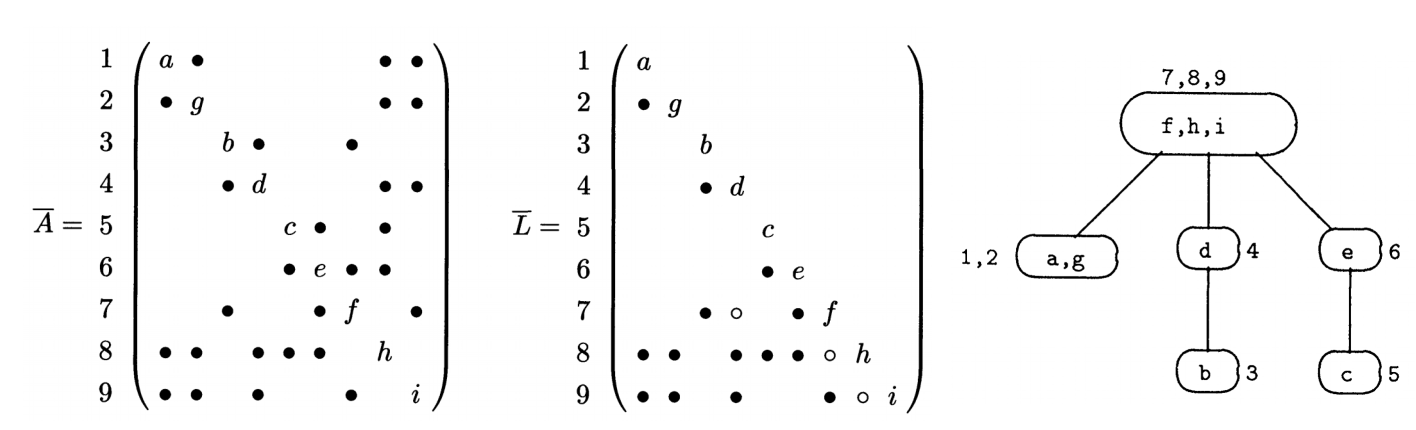
\includegraphics[width=1.0\textwidth]{figures/chapter-2/supernodal-method-postordering-and-etree.png}
\caption{An example of a supernodal elimination tree \cite{mult-frontal-original:2}}
\label{fig:supernodal-method-postordering-and-etree}
\end{figure}
 
 
Equation \ref{eq:mm-10} expresses the building process of a frontal matrix of a supernode. In contrast to \ref{eq:mm-9}, the frame matrix $\mathcal{F}_{j}$ contains more dense rows and columns. As before, we use \textit{extend-add} operation to get the full block update from children contribution matrices.\\


\todo{check grammar}
It should be mentioned there exist more sophisticated variants of supernodes. Most of the time, it intends to improve efficiency of the algorithm. \citeauthor{mult-frontal-original:2} pointed out that supernodes could be defined without using the contiguous constrains \cite{mult-frontal-original:2}. On another hand, \citeauthor{complexity-of-spdm} defines supernodes corresponded to separators from the nested dissection step  \cite{complexity-of-spdm} which was used for fill-in reduction.\\



 \begin{equation} \label{eq:mm-10}
	\mathcal{F}_{j} = \begin{bmatrix}a_{j,j} & a_{j,j+1} & \dots & a_{j,j+t}  & a_{j,i_1} & \dots & a_{j,i_r} \\
a_{j+1,j} & a_{j+1,j+1} & \dots & a_{j+1,j+t}  & a_{j+1,i_1} & \dots & a_{j+1,i_r} \\
\vdots & \vdots & \dots & \vdots \\
a_{j+t,j}  & a_{j+t,j+1} & \dots & a_{j+t,j+t}  & a_{j+t,i_1} & \dots & a_{j+t,i_r} \\
a_{i_1,j} & a_{i_1,j+1} & \dots & a_{i_1,j+t} \\
\vdots & \vdots & \dots & \vdots  & & 0\\ 
a_{i_r,j} & a_{i_r,j+1} & \dots & a_{i_r,j+t} \\
\end{bmatrix} \extendadd U_{c_1} \extendadd \dots \extendadd U_{c_s} 
\end{equation}


Up to this point we have already seen all key concepts of the multifrontal method and discussed how the algorithm works. We will move to the discussion of parallelization of the method. \\


The elimination tree, in fact, represents dependencies among columns. Conversely, the tree also shows independent steps of elimination process. Hence the tree forms independent problems that can be executed in parallel. Task parallelism is the main and primary source the algorithm parallelisation. Figure \ref{fig:elimination-tree-mm-parallel-steps} shows task parallelism, for the example given in Figure \ref{fig:supernodal-method-postordering-and-etree}, where each color represents a set concurrent tasks.\\


\figpointer{\ref{fig:elimination-tree-mm-parallel-steps}}

\begin{figure}[htpb]
  \centering
  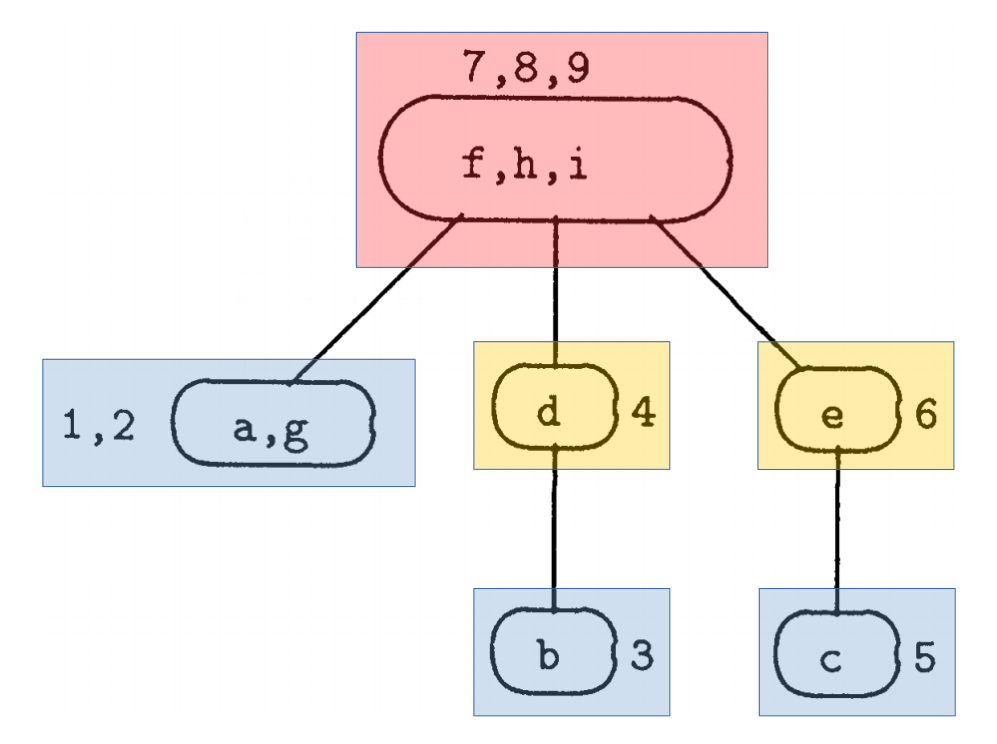
\includegraphics[width=0.5\textwidth]{figures/chapter-2/elimination-tree-parallel.png}
\caption{Parallel steps of the multifrontal method based on the example in Figures \ref{fig:supernodal-method-postordering-and-etree}}
\label{fig:elimination-tree-mm-parallel-steps}
\end{figure}


For example, nodes on separate branches of the tree are totally independent and can processed in parallel. However, as soon as at least two branches run into the same node it forms a dependency and we have to wait all contribution matrices of its children and cannot proceed further.\\ 


We can observe the amount of task parallelism is rapidly decreasing while moving towards the root along the tree. Once we reach the root of the tree the algorithm becomes totally sequential. This fact can play the significant role in strong scaling behavior of the method.\\


We developed two simple models based on perfectly balanced binary trees to better understand strong scaling of the algorithm. The main concept of the models is so-called cost per level or cost per node. This idea is similar to the recursion trees in \cite{recursion-tree} which explains and computes complexity of recurrent algorithms.\\


Figure \ref{fig:mm-parallel-model-tree-linear} represents the first model where we keep the same cost per level whereas the second model (Figure \ref{fig:mm-parallel-model-tree-quadratic}) simulates quadratic cost decay from level to level. Additionally we assume that computational cost distributed uniformly between nodes at the same level for both models.\\


\figpointer{\ref{fig:mm-parallel-model-tree}}
\begin{figure}
\centering
	\begin{tabular}{cc}
			\subfloat[Model 1: equal cost per level]{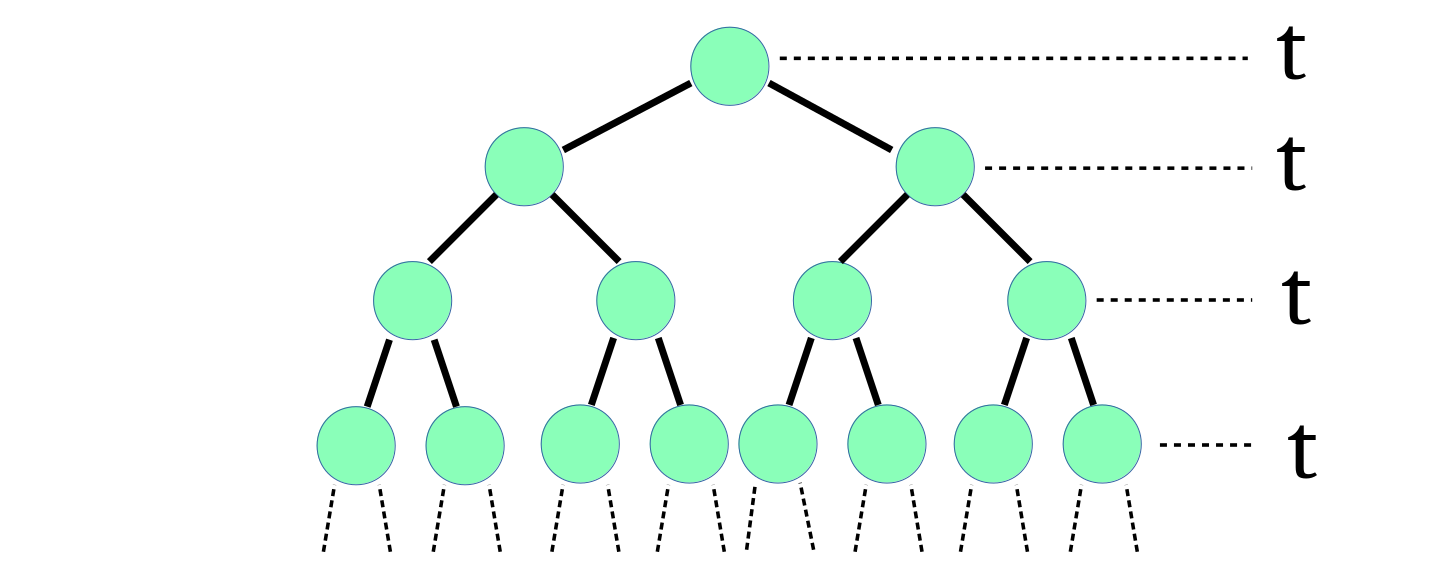
\includegraphics[width=0.5\textwidth]{figures/chapter-2/mm-parallel-model-tree-1.png} \label{fig:mm-parallel-model-tree-linear}} & 
		\subfloat[Model 2: quadratically decreasing cost per level]{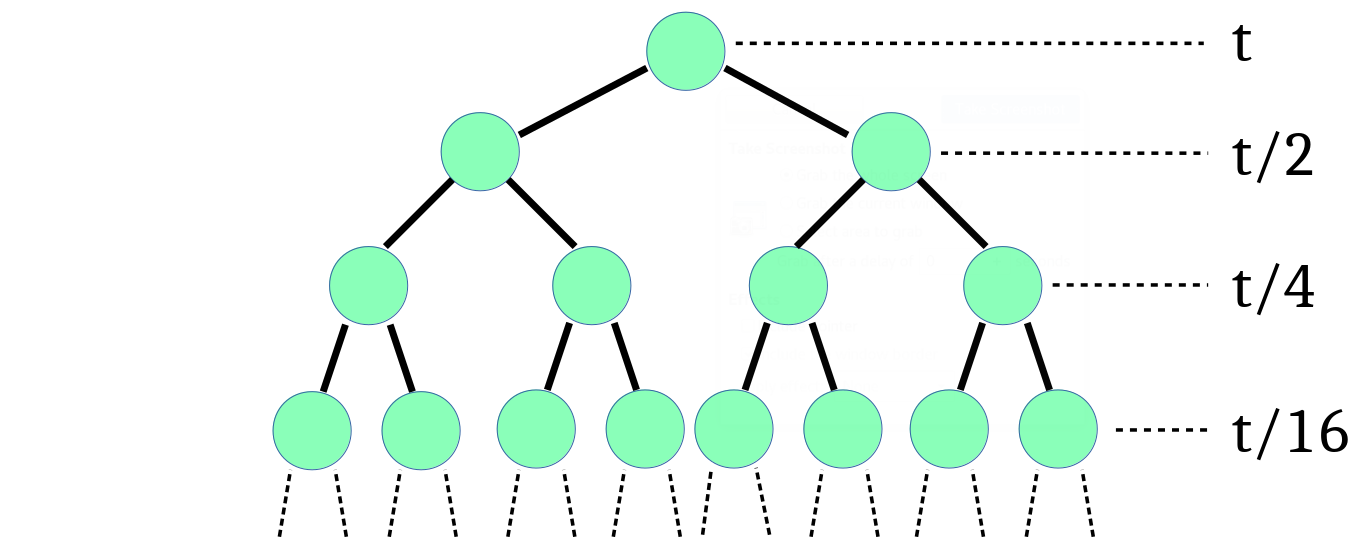
\includegraphics[width=0.5\textwidth]{figures/chapter-2/mm-parallel-model-tree-2.png} \label{fig:mm-parallel-model-tree-quadratic}} \\
	\end{tabular}
	\caption{Simple parallel models of the multifrontal method}
	\label{fig:mm-parallel-model-tree}
\end{figure}

\todo{sentence refactoring}
We have to say that our models mimic only numerical factorization and do not include time spent on any per-processing steps, for example, fill-in reduction reodering. A cost per level can be interpreted in different ways e.g. increase of partial factorization time due to growth of frontal matrices in size, time increase spent on numerical pivoting, increase of MPI communication overheads due to growth of contribution matrices, etc. It should be mentioned that real computer implementations of the multifrontal algorithm (MUMPS, SuperLU, etc.) are quite sophisticated in many aspects and our models do not have any intention to analyze performance of a particular package. Instead the objective of these models is to show possible strong scaling behavior and possible bottlenecks. \\


We will consider only task parallelism at the beginning to a first approximation and later we will discuss how additional data parallelism can affect algorithm performance.\\

% assumtion that cost is equal within the level!!!

Instead of coloring given in Figure \ref{fig:elimination-tree-mm-parallel-steps}, we assume that each level has the same color and thus can be executed fully in parallel if we have enough processing elements. We cannot go to the next level till the current one has not been completed yet i.e. free processing elements, that do not have nodes to execute at the current level, have to wait.\\


As we mentioned above the root of the tree can be processed purely sequentially if we only consider task parallelism. As a first approximation, time spent on the root factorization determines the minimal execution time according to the Amdahl's low \cite{wiki:amdahls-low}. More precisely, the minimal execution time is equal to a sum of time spent on single node partial factorization at each level. This time determines the asymptote on the corresponding speed-up graph.\\


We considered a perfectly balanced tree with 16 levels, 65535 nodes and the maximum of 20 processing elements as an example. The numerical results of linear and quadratic models can be viewed in Figures \ref{fig:mm-parallel-model-tree-linear} and \ref{fig:mm-parallel-model-tree-quadratic}, respectively. The figures show a rapid drop of performance, especially in case of the quadratic model. Table \ref{table:mm-potential-model-speed-up} demonstrates the maximum potential speed-up, having 32768 processing elements which is equal to the number of leaves of the tree, against the speed-up we have got using only 20 processing elements.\\


\figpointer{\ref{fig:mm-parallel-model-speed-up}}
\begin{figure}
\centering
	\begin{tabular}{cc}
			\subfloat[Theoretical speed-up of Model 1]{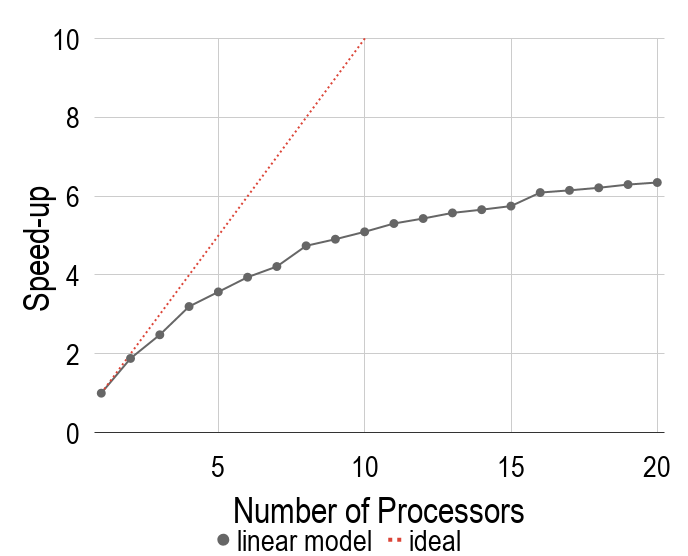
\includegraphics[width=0.45\textwidth]{figures/chapter-2/mm-parallel-model-tree-1-speedup.png}} &
		\subfloat[Theoretical speed-up of Model 2]{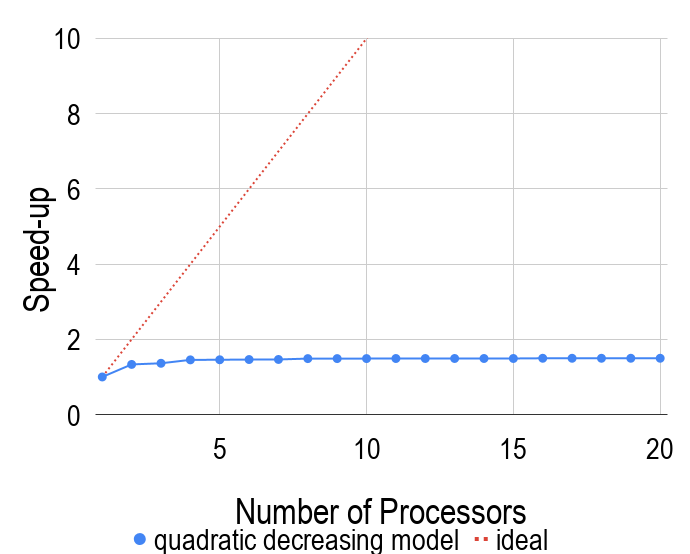
\includegraphics[width=0.45\textwidth]{figures/chapter-2/mm-parallel-model-tree-2-speedup.png}} \\
	\end{tabular}
	\caption{Theoretical speed-up}
	\label{fig:mm-parallel-model-speed-up}
\end{figure}


\begin{table}[htpb]
\centering
\begin{tabular}{|c|c|c|}
\hline
        & 20 PEs  & 32768 PEs \\ \hline
Model 1 & 6.3492  & 8.0000    \\ \hline
Model 2 & 1.4972 & 1.5000   \\ \hline
\end{tabular}
\caption{Potential speed-up of linear and quadratic models}
\label{table:mm-potential-model-speed-up}
\end{table}


We can see that model 1 still has some potential to grow whereas the second model has already reached its asymptote and further increase of processing elements does not make sense. In spite of a potential growth of the first model, both models have very low parallel efficiency even with 20 processing elements which can be observed from table \ref{table:mm-model-efficiency-20-pe}.\\


\begin{table}[htpb]
\centering
\begin{tabular}{|c|c|}
\hline
        & 20 PEs \\ \hline
Model 1 & 0.3175 \\ \hline
Model 2 & 0.0749 \\ \hline
\end{tabular}
\caption{Efficiency of linear and quadratic models using 20 PEs}
\label{table:mm-model-efficiency-20-pe}
\end{table}


Both models shows that computational intensity per node grows from bottom to top. It is easy to conclude from Figure \ref{fig:mm-parallel-model-tree} that intensity per node is equal $t/2^{i}$ and $t/2^{2i}$ for the first and second models, respectively (where $i$ is a level of the tree). It reflects that the most intensive part of the method is centered on the top part of the tree i.e. first few level. \citeauthor{mult-frontal-original:2} discussed application of the multifrontal method to a $k-by-k$ regular model problem with nine-point difference operator in his paper \cite{mult-frontal-original:2}. He observed that factorization of the last 6 nodes took slightly more than 25\% of the total amount of arithmetical operations. As a comparison, table \ref{table:mm-simple-model-work-load} shows fractions of time spent on processing first few top levels of our models: 1 and 2.\\


\begin{table}[htpb]
\centering
\begin{tabular}{|c|c|c|}
\hline
        & Model 1 & Model 2 \\ \hline
Level 0 & 6.25\%  & 50.00\% \\ \hline
Level 1 & 12.50\% & 75.00\% \\ \hline
Level 2 & 18.75\% & 87.50\% \\ \hline

\end{tabular}
\caption{Distribution workload per level in case model 1 and 2}
\label{table:mm-simple-model-work-load}
\end{table}


As we can see, the result of our first model is relatively close to 25\% and, therefore, it looks quite optimistic. However, the second model shows that 87\% of workload is focused on the top part of the tree and, as a result, we can consider that model as extremely pessimistic. \\


By and large, reduction of time spent on the top nodes is a way to improve strong scaling behavior. To do so, data parallelism can be additionally exploited for these nodes. It is worth noting that data parallelism at bottom levels does not make sense because it leads to increase of granularity there and thus increase communication overheads which can lead to significant performance drop.\\


Figure \ref{fig:mumps-task-data-parallelism} shows an example of two types of parallelism applied to the algorithm. First of all, we can see the leaves are grouped in subtrees and a single PE is assigned to each subtree. Other nodes are distributed among three different types. Nodes of the first type uses task parallelism only, which is induced by the tree, and each node is executed in a single processor. The second type exploits data parallelism with 1D block row distribution among the processors. The root belongs to the third type where data parallelism is used with 2D block cyclic distribution. The details of MUMPS parallelism management is carefully explained and can be found in \cite{mumps:task-data-parallelism}.\\


\figpointer{\ref{fig:mumps-task-data-parallelism}}

\begin{figure}[htpb]
  \centering
  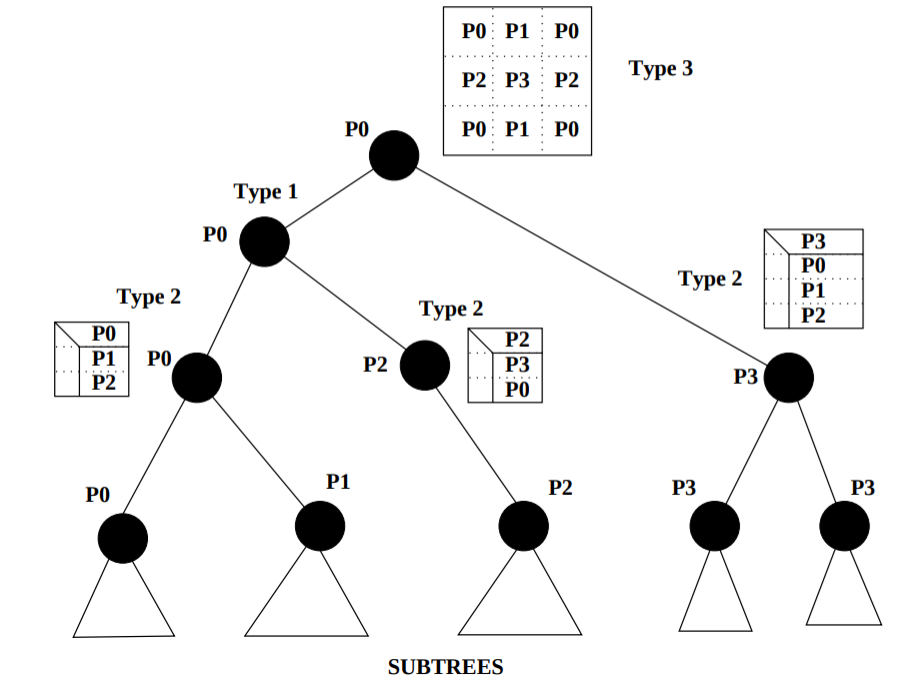
\includegraphics[width=0.65\textwidth]{figures/chapter-2/mumps-task-data-parallelism.png}
\caption{MUMPS parallelism management in case of 4 PEs \cite{mumps:task-data-parallelism}}
\label{fig:mumps-task-data-parallelism}
\end{figure}


All the techniques mentioned above were designed to improve strong scaling behavior by splitting the most intensive parts among all available processors. Going back to our models, we can also think about that in a slightly different way, namely: \textit{data parallelism helps to re-distribute cost per node/level on the corresponding elimination tree}. However, we have to notice that efficiency of data parallelism totally depends on sizes of frontal matrices at the top part of the tree. In case of skinny sparse matrices, oversubscription of processing elements can lead to strong performance penalties as we could see from section \ref{subseq:direct methods}. A machine-dependent minimal frontal matrix size was introduced in MUMPS in order to control whether to use ScaLAPACK at the root node or not \cite{mumps-manual}. It can happen that the algorithm uses only task parallelism, due to the threshold, and, as a results, scaling will only depend on the tree structure that can be deep and unbalanced.\\


Figure \ref{fig:model-1-vs-mumps} shows comparison of strong scaling between model 1 and parallel numerical factorization of the matrix \textit{\textbf{memchip}} (Table \ref{table:suite-sparse-matrix-set}) done with using MUMPS library. The sparsity pattern before and after fill-in reduction is shown in figure \ref{fig:memchip-matrix-sparsity-pattern}. 

\todo{add some examples to the appendix}
\figpointer{\ref{fig:model-1-vs-mumps}. Show standard deviation}
\begin{figure}[htpb]
  \centering
  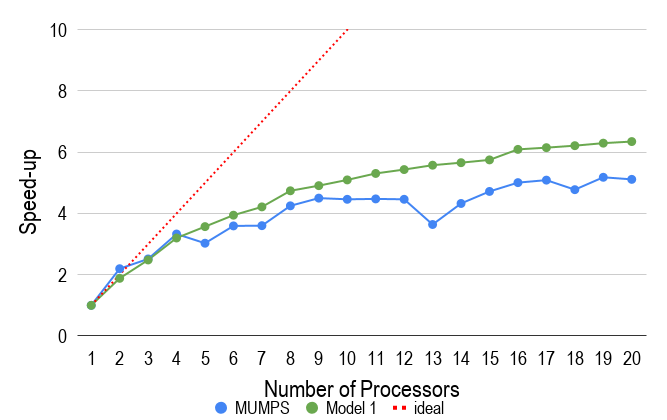
\includegraphics[width=0.65\textwidth]{figures/chapter-2/model-1-vs-mumps.png}
\caption{Comparison between model 1 and numerical factorization of the matrix \textit{\textbf{memchip}} using MUMPS library}
\label{fig:model-1-vs-mumps}
\end{figure}


\figpointer{\ref{fig:memchip-matrix-sparsity-pattern}}
\begin{figure}[htpb]
  \centering
  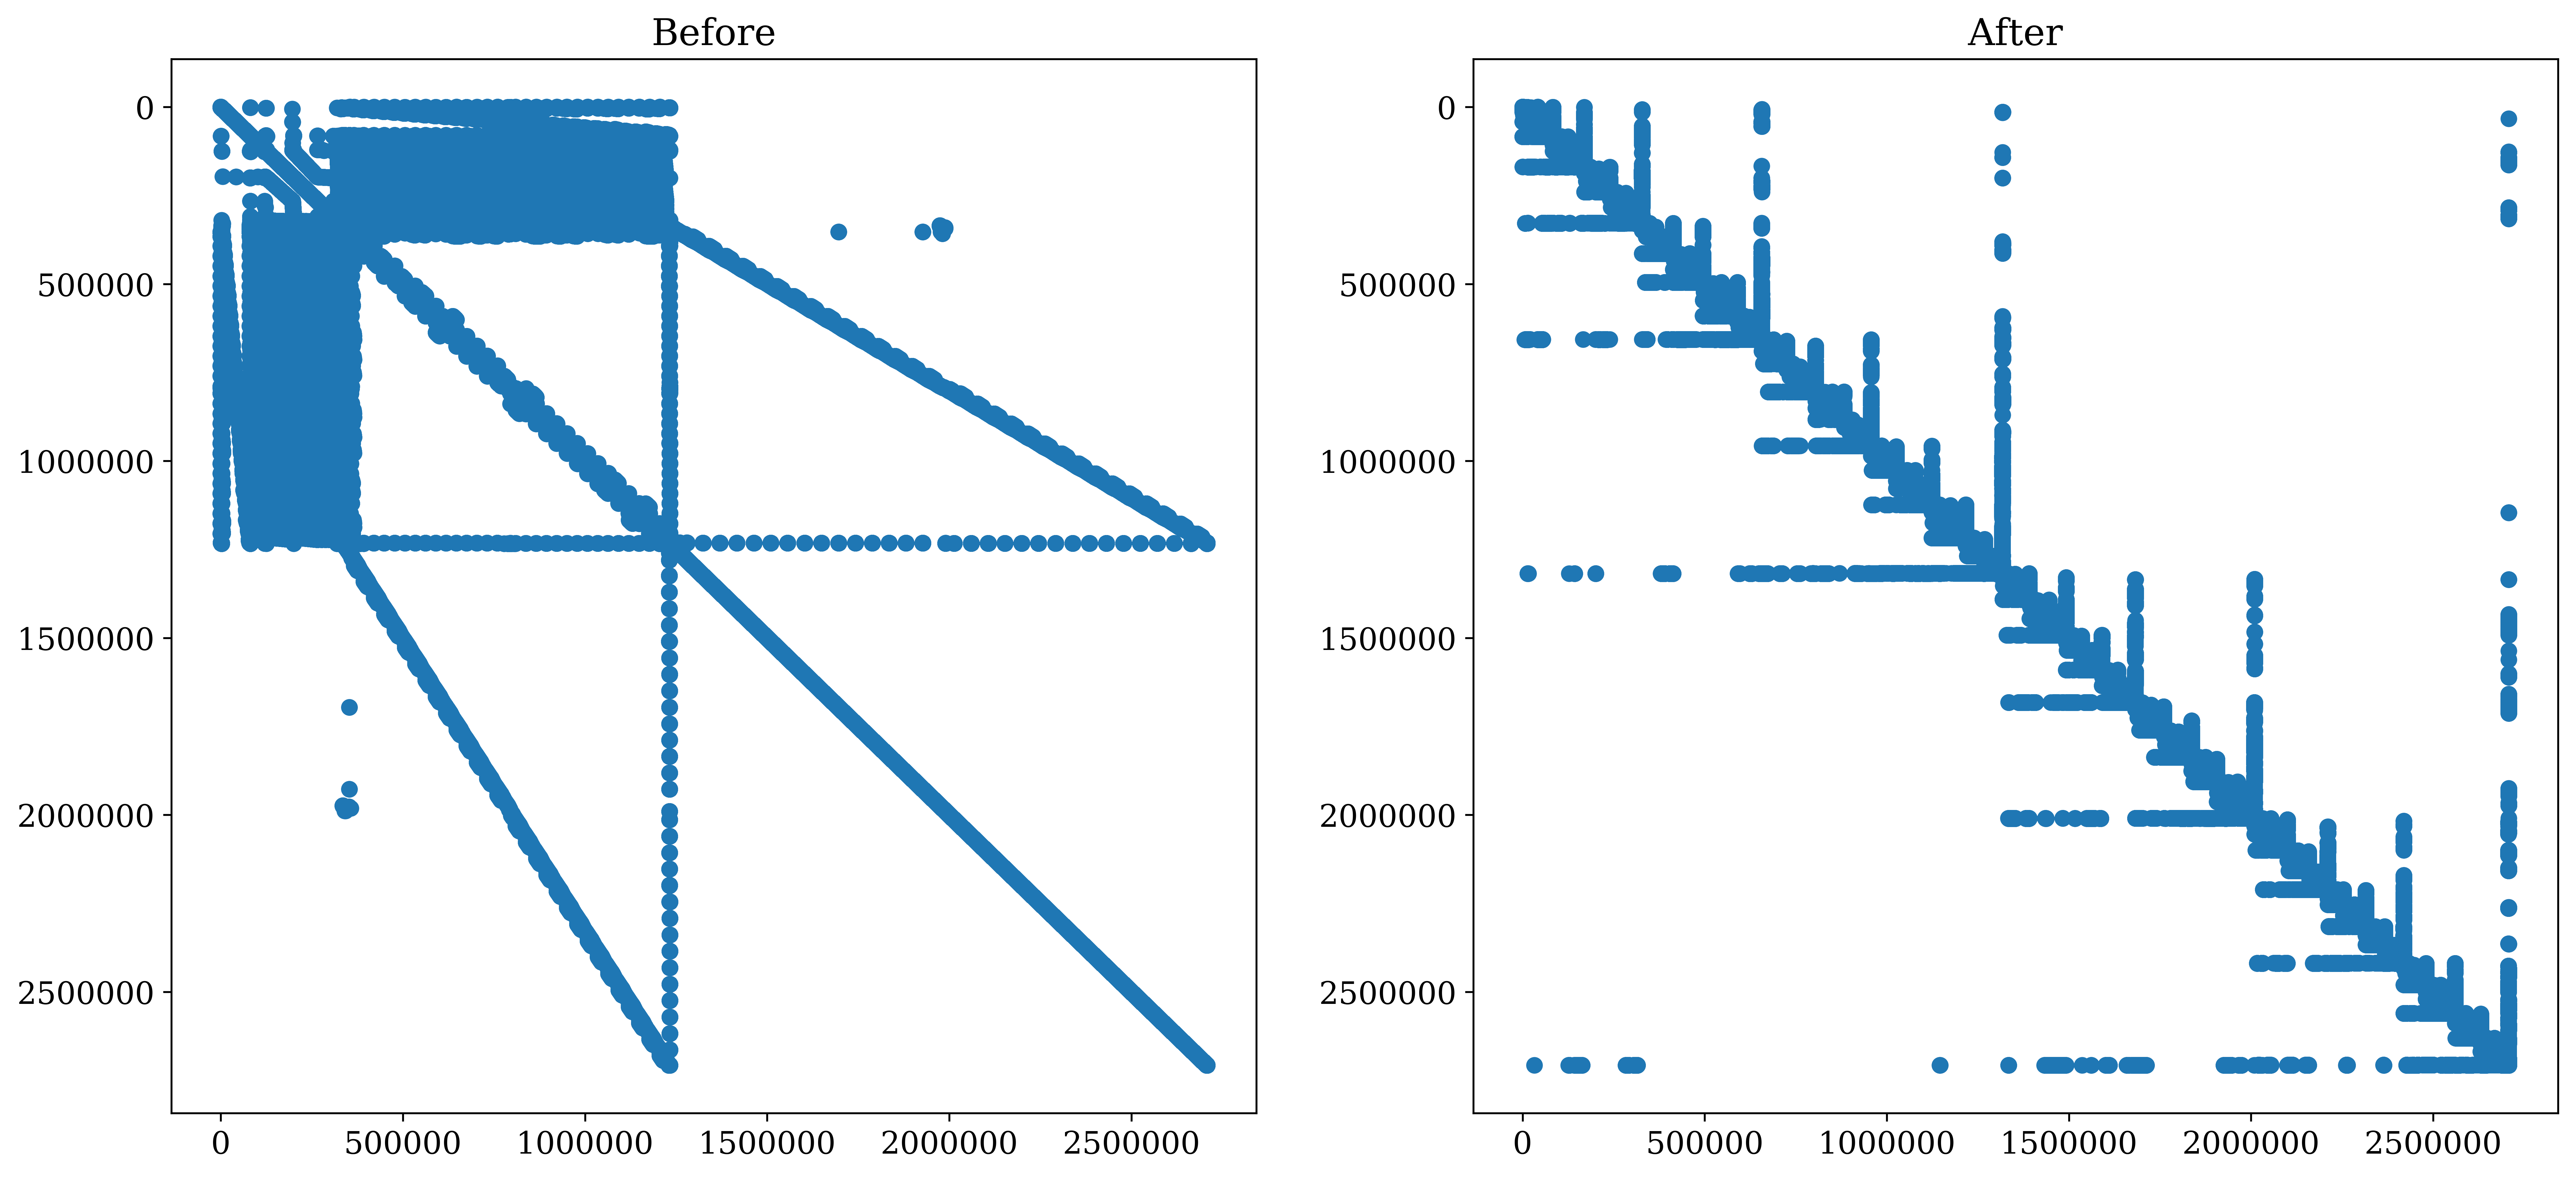
\includegraphics[width=1.00\textwidth]{figures/chapter-2/memchip-matrix-sparsity-pattern.png}
\caption{Sparsity structure of the matrix \textit{\textbf{memchip}} before and after fill-in reduction}
\label{fig:memchip-matrix-sparsity-pattern}
\end{figure}




As we can see, our model and the experiment show the same trend and the results are pretty much close to each other. However, our model takes into consideration only task parallelism whereas MUMPS exploits both data and task parallelism. Additionally, we have to mention that our model 1 works well only for relatively big sparse matrices. It can be quite inaccurate in case of small/skinny sparse systems. \\


In general, it is possible to refine our models and make them more accurate, using Bulk Synchronous Parallel (BSP) approach, for example. However, it will require to possess a real postordered elimination tree, extracted from a specific implementation of multifrontal method, together with information about supernodes sizes. We strongly believe the new enhanced model can explain the jagged strong scaling behavior of the MUMPS solver that we can observe in figure \ref{fig:model-1-vs-mumps}. But, this approach seems to be quite cumbersome and requires to delve into the source code of a particular library. It is needless to say that data can be retrieved only during run time and only after the analysis phase. This makes it less valuable and we can see that it is definitely a wrong way to go.\\


There are few important aspects to discuss at the end of the section. Numerical robustness is the main advantage of the multifrontal method. It does not require any preconditioner to solve a system of equations. As we discussed in the previous section, tuning a specific preconditioning algorithm can take a considerable amount of time, especially in case of our systems. As another advantage, the method (heavily) exploits matrix sparsity which lowers computational complexity up to $O(n^2)$. In case of massively huge matrices, the algorithm can utilize the secondary memory which sometimes is only one way to solve a system.\\


We can conclude, from the analysis above, the method has inherently bad scaling behavior and it is quite sensitive to a matrix structure. We will see later that it is almost impossible to predict the saturation point i.e. a point after which performance either drops or stays at the same level. We assume that scaling becomes better with growth of a matrix size. However, we cannot expect such behavior for small and medium systems.\\  


Secondly, we can see the algorithm requires many pre-processing steps to be done before numerical factorization phase. All these steps must run in parallel and be highly scalable. Apart from performance constrains of the steps, they must lead to wide and well balanced elimination trees which becomes crucial during the numerical phase.\\


Lastly, the algorithm can fail due to incorrect  working space prediction. As a results, factorization has to be restarted with some modification of input solver parameters.\\



\label{subseq:hybrid-method-description}

Nowadays, iterative methods is a common choice for solving sparse systems of linear equations because of their possible fast convergence and high parallel efficiency. However, application of such method always demands preconditioning of ill-conditioned systems to make methods converge to numerical accurate solutions. It can be clearly observed from table \ref{table:grs-matrix-set} that numerical integration of thermo-hydraulic simulations in \gls{athlet} entails solving such ill-conditioned systems  based on estimated condition numbers of matrices form \gls{grs} matrix set.\\


As the first step of the study, we tested various preconditioning algorithms together with their tuning parameters, mentioned in table \ref{table:preconditioners}, applied to \gls{grs} matrix set. \gls{gmres} was chosen as an iterative solver with values of relative and absolute convergence tolerances in the residual norm to be equal to $1E-8$ and $1E-4$, respectively. A coarse grid search was used with maximum 3 values for each tuning parameter starting from the default towards more accurate values in order to refine settings of each preconditioning algorithm. Testing results showed that none of them could lead to convergence for the entire set of matrices.\\


One can assume that a finer grid search can result in finding a suitable preconditioning algorithm with settings that can lead to convergence of \gls{gmres} solver for the entire set. However, it is important to point out the matrices were generated by running the most common \gls{grs} thermo-hydraulic test-scenarios and saving them somewhere during the time integration process. Hence, there is no guarantee that the settings found in such a way can always lead to convergence of \gls{gmres} solver in all time steps of any thermo-hydraulic simulation. Therefore, iterative methods may not satisfy \textit{robustness} criteria stated in chapter \ref{chapter:problem-statment} as a non-functional requirement to the time integration solver used in \gls{athlet}.\\


Taking into account the above reasoning, we have come to the conclusion that sparse direct methods is the best choice for our problem, in spite of the limited tree-task parallelism described in subsection \ref{subseq:direct-parallel-aspects}, because the methods stably result in numerical accurate solutions even in case of ill-conditioned linear systems. Hence, the next objective of the study is to find a suitable sparse direct method and its implementation, and adapt it for \gls{hw1} compute-cluster environment in terms of efficient parallel execution. \\



\label{subseq:mm-library-choice}

Fair to say, there is no single algorithm or software that is the best for all types of linear systems \cite{list-of-sparse-direct-solvers}.\\


Nowadays, there exist many different avaliable sparse direct solvers. Some of them are tunned for specific linear systems whereas others are targeted for the most general cases \cite{list-of-sparse-direct-solvers}. Some of them handle tree-task and node-data parallelism in different ways even within the same library depending on sizes of frontal matrices and other criteria \cite{wsmp}, \cite{mumps-manual}, \cite{superlu-manual}. Hence, parallel performance of a direct sparse method depends heavily on its specific implementation. Table \ref{table:mm-library-spec} represents a short summary of almost all available libraries capable to run on distributed-memory machines, at the time of writing, based on works \cite{list-of-sparse-direct-solvers} and \cite{petsc-web-page}.\\


\begin{table}[ht]
\small
\centering
\begin{tabular}{|c|c|c|c|c|}
\hline
Package & Method             & Matrix Types                 & \multicolumn{1}{c|}{\begin{tabular}[c]{@{}c@{}}PETSc\\ Interface\end{tabular}} & License      \\ \hline
Clique       & Multifrontal       & Symmetric      & \multicolumn{1}{c|}{\begin{tabular}[c]{@{}c@{}}Not \\ Officially\end{tabular}} & Open  \\ \hline
MF2          & Multifrontal       & \begin{tabular}[c]{@{}c@{}}Symmetric\\ pattern\end{tabular} & No              & -            \\ \hline
DSCPACK      & Multifrontal       & SPD                          & No              & Open* \\ \hline
MUMPS        & Multifrontal       & General                      & Yes             & Open  \\ \hline
PaStiX       & Left looking & General                      & Yes             & Open  \\ \hline
PSPASES      & Multifrontal       & SPD                          & No              & Open* \\ \hline
SPOOLES      & Left-looking       & \begin{tabular}[c]{@{}c@{}}Symmetric\\ pattern\end{tabular} & No              & Open* \\ \hline
SuperLU\_DIST & Right-looking      & General                      & Yes             & Open  \\ \hline
symPACK      & Left-Right looking & SPD                          & No              & Open  \\ \hline
S+           & Right-lookin       & General                      & No              & -            \\ \hline

PARDISO         & Multifrontal       & General                      & No              & Commercial   \\ \hline

WSMP         & Multifrontal       & General                      & No              & Commercial   \\ \hline
\end{tabular}
\caption{A list of direct sparse linear solvers adapted for distributed-memory computations, \cite{list-of-sparse-direct-solvers}, \cite{petsc-web-page}.\\}
where SPD - Symmetric Positive Definite; 
Open* - an interface is not officially supported by the \acrshort{petsc} team
\label{table:mm-library-spec}
\end{table}


It can be clearly observed, from Table \ref{table:mm-library-spec}, that only \acrshort{mumps}, PaStiX and SuperLU\_DIST cover all requirements induced by \acrshort{grs}, see Chapter \ref{chapter:problem-statment}, in particular: open-source license and a direct interface to \acrshort{petsc}. It is interesting to notice that all libraries, mentioned above, are implementations of different sparse direct methods, namely: multi-frontal (\acrshort{mumps}), left-looking (PaStiX) and right-locking (SuperLU\_DIST). Moreover, PaStiX and SuperLU\_DIST use only static pivoting \cite{pastix-manual}, \cite{superlu-manual} whereas \acrshort{mumps} provides a full implementation of the threshold pivoting strategy \cite{mumps-manual}, described in Subsection \ref{subseq:pivot-hadling}.\\


To compare the libraries, a couple of flat-\acrshort{mpi} tests were performed using \acrshort{grs} matrix set on \gls{hw1} machine. \acrshort{petsc} library was compiled and configured with \acrshort{mumps} (version 5.1.2), PasTiX (version 6.0.0) and SuperLU\_DIST (version 5.4) packages using their default parameter settings. An internal built-in \acrshort{petsc} profiler was used to measure execution time.  A time limit of 15 minutes was set up for each test-case to prevent blocking of a cluster compute-node from an unexpected long program execution. Results are summarized in Tables \ref{table:lc-cube-5-result}, \ref{table:lc-cube-64-result}, \ref{table:lc-k3-18-result} and in appendix \ref{app:app-lc} where numerical values are given in seconds.\\



\begin{table}[ht]
\centering
\begin{tabular}{|c|c|c|c|l|c|c|c|c|}
\cline{1-4} \cline{6-9}
MPI & MUMPS    & PaStiX   & SuperLU  &  & MPI & MUMPS    & PaStiX   & SuperLU  \\ \cline{1-4} \cline{6-9} 
1   & 7.02E-02 & 8.72E-02 & 3.17E+00 &  & 11  & 7.55E-02 & 8.89E-02 & 5.82E-01 \\ \cline{1-4} \cline{6-9} 
2   & 6.73E-02 & 7.10E-02 & 1.43E+00 &  & 12  & 7.61E-02 & 1.06E-01 & 4.37E-01 \\ \cline{1-4} \cline{6-9} 
3   & 6.36E-02 & 7.01E-02 & 1.07E+00 &  & 13  & 7.84E-02 & 9.72E-02 & 5.43E-01 \\ \cline{1-4} \cline{6-9} 
4   & 6.28E-02 & 7.11E-02 & 8.17E-01 &  & 14  & 8.06E-02 & 1.02E-01 & 4.22E-01 \\ \cline{1-4} \cline{6-9} 
5   & 6.50E-02 & 7.15E-02 & 7.51E-01 &  & 15  & 8.20E-02 & 1.19E-01 & 3.91E-01 \\ \cline{1-4} \cline{6-9} 
6   & 6.72E-02 & 7.62E-02 & 6.15E-01 &  & 16  & 8.07E-02 & 1.19E-01 & 4.44E-01 \\ \cline{1-4} \cline{6-9} 
7   & 6.91E-02 & 7.69E-02 & 6.48E-01 &  & 17  & 8.38E-02 & 1.22E-01 & 5.19E-01 \\ \cline{1-4} \cline{6-9} 
8   & 6.89E-02 & 8.17E-02 & 5.41E-01 &  & 18  & 8.40E-02 & 1.26E-01 & 3.77E-01 \\ \cline{1-4} \cline{6-9} 
9   & 7.50E-02 & 8.28E-02 & 5.02E-01 &  & 19  & 8.58E-02 & 1.33E-01 & 5.47E-01 \\ \cline{1-4} \cline{6-9} 
10  & 7.22E-02 & 8.52E-02 & 4.64E-01 &  & 20  & 8.64E-02 & 1.49E-01 & 3.39E-01 \\ \cline{1-4} \cline{6-9} 
\end{tabular}
\caption{Comparisons of parallel performance of  \textit{cube-5} matrix factorization using \acrshort{mumps}, PasTiX and SuperLU\_DIST solvers with their default parameter settings}
\label{table:lc-cube-5-result}
\end{table}


\begin{table}[ht]
\centering
\begin{tabular}{|c|c|c|c|l|c|c|c|c|}
\cline{1-4} \cline{6-9}
MPI & MUMPS    & PaStiX   & SuperLU  &  & MPI & MUMPS    & PaStiX   & SuperLU  \\ \cline{1-4} \cline{6-9} 
1   & 1.36E+00 & 1.39E+00 & time-out &  & 11  & 7.75E-01 & 8.15E-01 & time-out \\ \cline{1-4} \cline{6-9} 
2   & 1.00E+00 & 9.82E-01 & time-out &  & 12  & 7.81E-01 & 8.10E-01 & time-out \\ \cline{1-4} \cline{6-9} 
3   & 8.83E-01 & 1.06E+00 & time-out &  & 13  & 7.85E-01 & 8.35E-01 & time-out \\ \cline{1-4} \cline{6-9} 
4   & 8.17E-01 & 8.74E-01 & time-out &  & 14  & 7.85E-01 & 8.18E-01 & time-out \\ \cline{1-4} \cline{6-9} 
5   & 7.85E-01 & 8.50E-01 & time-out &  & 15  & 7.88E-01 & 8.46E-01 & time-out \\ \cline{1-4} \cline{6-9} 
6   & 8.06E-01 & 8.52E-01 & time-out &  & 16  & 7.81E-01 & 8.23E-01 & time-out \\ \cline{1-4} \cline{6-9} 
7   & 7.71E-01 & 8.33E-01 & time-out &  & 17  & 6.83E-01 & 8.49E-01 & time-out \\ \cline{1-4} \cline{6-9} 
8   & 7.66E-01 & 8.33E-01 & time-out &  & 18  & 7.96E-01 & 8.44E-01 & time-out \\ \cline{1-4} \cline{6-9} 
9   & 7.93E-01 & 8.35E-01 & time-out &  & 19  & 8.04E-01 & 8.65E-01 & time-out \\ \cline{1-4} \cline{6-9} 
10  & 8.07E-01 & 8.15E-01 & time-out &  & 20  & 6.85E-01 & 8.87E-01 & time-out \\ \cline{1-4} \cline{6-9} 
\end{tabular}
\caption{Comparisons of parallel performance of  \textit{cube-64} matrix factorization using \acrshort{mumps}, PasTiX and SuperLU\_DIST solvers with their default parameter settings}
\label{table:lc-cube-64-result}
\end{table}


\begin{table}[h!]
\centering
\begin{tabular}{|c|c|c|c|l|c|c|c|c|}
\cline{1-4} \cline{6-9}
MPI & MUMPS    & PaStiX   & SuperLU &  & MPI & MUMPS    & PaStiX   & SuperLU \\ \cline{1-4} \cline{6-9} 
1   & 1.55E+02 & 6.44E+01 & crashed &  & 11  & 1.77E+01 & 3.81E+01 & crashed \\ \cline{1-4} \cline{6-9} 
2   & 6.28E+01 & 4.84E+01 & crashed &  & 12  & 1.60E+01 & 3.75E+01 & crashed \\ \cline{1-4} \cline{6-9} 
3   & 5.06E+01 & 5.02E+01 & crashed &  & 13  & 1.42E+01 & 3.58E+01 & crashed \\ \cline{1-4} \cline{6-9} 
4   & 4.17E+01 & 4.50E+01 & crashed &  & 14  & 1.45E+01 & 3.59E+01 & crashed \\ \cline{1-4} \cline{6-9} 
5   & 2.52E+01 & 3.98E+01 & crashed &  & 15  & 1.47E+01 & 3.57E+01 & crashed \\ \cline{1-4} \cline{6-9} 
6   & 2.58E+01 & 4.29E+01 & crashed &  & 16  & 1.41E+01 & 3.52E+01 & crashed \\ \cline{1-4} \cline{6-9} 
7   & 2.65E+01 & 4.30E+01 & crashed &  & 17  & 1.54E+01 & 3.45E+01 & crashed \\ \cline{1-4} \cline{6-9} 
8   & 2.59E+01 & 3.73E+01 & crashed &  & 18  & 1.52E+01 & 3.31E+01 & crashed \\ \cline{1-4} \cline{6-9} 
9   & 1.95E+01 & 4.08E+01 & crashed &  & 19  & 1.52E+01 & 3.31E+01 & crashed \\ \cline{1-4} \cline{6-9} 
10  & 1.91E+01 & 3.81E+01 & crashed &  & 20  & 1.38E+01 & 3.16E+01 & crashed \\ \cline{1-4} \cline{6-9} 
\end{tabular}
\caption{Comparisons of parallel performance of \textit{k3-18} matrix factorization using \acrshort{mumps}, PasTiX and SuperLU\_DIST solvers with their default parameter settings}
\label{table:lc-k3-18-result}
\end{table}



Some problems were detected during  SuperLU\_DIST library testing. First of all, executions of \textit{cube-64} and \textit{k3-2} test-cases exceeded the set time limit. Secondly, it was noticed the library was crashing during processing of \textit{k3-18}, \textit{cube-645} and (partially) \textit{pwr-3d} test-cases. Debugging revealed that a segmentation fault occurred in function \textit{pdgstrf}  during the numerical factorization phase. Nonetheless, it is still unclear whether the problem was software or hardware specific. A solution or a reason of such program behavior has not been found at the moment of writing.\\


% FOR PRESENTATION: it can be due to wrong matrix representation in binary \acrshort{petsc} files. I ran into the same problem with METIS when it spinned the CPU for hours due to wrong CRS format

To complete comparison and evaluate parallel performance SuperLU\_DIST library, an additional test was conducted using a 2D formulation of the Poisson problem with \textit{100000} unknown. According to the results, SuperLU\_DIST managed to complete matrix factorizations within the set time limit without crashing, however, it showed abnormal jagged strong scaling behavior. Moreover, it turned out it was the slowest in comparison to the other solvers. The results are shown in Figure \ref{fig:5-point-stencil-solvers-comparison}.\\



\figpointer{\ref{fig:5-point-stencil-solvers-comparison}}
\begin{figure}[htpb]
  \centering
  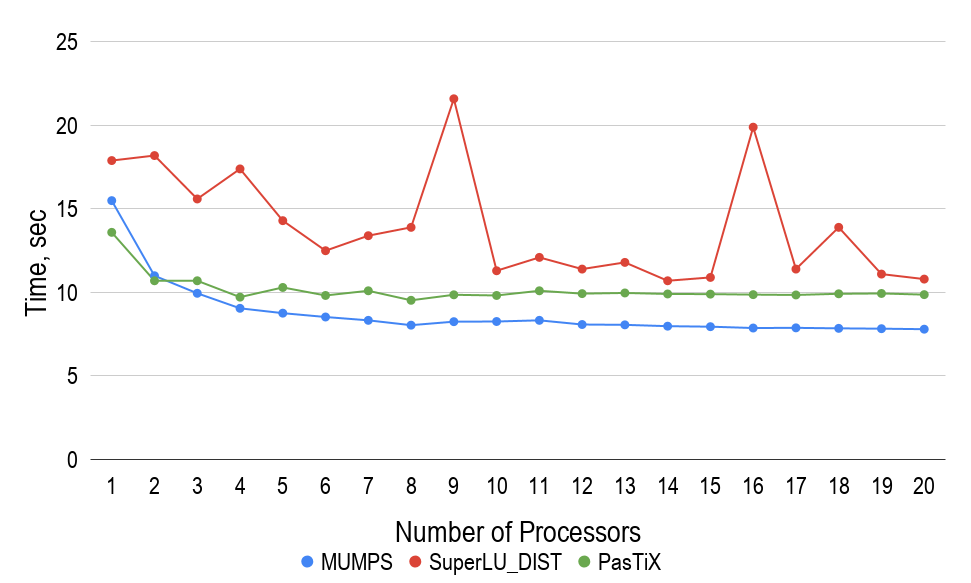
\includegraphics[width=0.85\textwidth]{figures/chapter-2/solvers-comparison-5-point-stencil.png}
\caption{Comparisons of parallel performance of 5 point-stencil Poisson matrix (1000000  equations) factorization using 
\acrshort{mumps}, PasTiX and SuperLU\_DIST libraries with their default parameter settings}
\label{fig:5-point-stencil-solvers-comparison}
\end{figure}

% FOR PRESENTATION: we think that 

According to the initial and additional tests, \acrshort{mumps} library showed the best parallel performance and scaling in contrast to the other solvers. No abnormal behavior during its operation was detected. In some cases, it only required to increase a multiplicative factor of estimated working space which was used to hold frontal matrices and factors $L$ and $U$ in memory. PaStiX was the second fastest solver according to the results of testing. However,  it was often considerably slower than \acrshort{mumps}. At the same time, SuperLU\_DIST showed the worst results. Additionally, as it was mentioned above, we experienced some technical problems during operation of this library.\\


A literature review showed quite contradictory results and conclusions. For example, \citeauthor{wsmp}, in work \cite{wsmp}, came to nearly the same outcome, as we did, comparing parallel performance of WSMP, \acrshort{mumps} and SuperLU\_DIST libraries using their matrix set. However, \citeauthor{mm-comparison-of-packages} showed, in \cite{mm-comparison-of-packages}, that SuperLU\_DIST spent the least amount of time on solving  systems of linear equations in contrast to the other solvers used in their work. It needless to say that both research groups used different matrix sets and hardware. Nevertheless, it reveals a quite important fact that a selection of a particular method and its implementation can depend heavily on a specific matrix set.\\


In this section, we compared different sparse direct methods and their concrete implementations using their default parameter settings with regard to \acrshort{grs} matrix set. Based on the obtained results and literature review, \acrshort{mumps} library was chosen for the following study. In Section \ref{subseq:mumps-review}, we make an overview of the library and its specific traits. \\



\subsection{Review of MUMPS Library}
\label{subseq:mumps-review}

\todo{read comments}
%All the techniques mentioned above were designed to improve strong scaling behavior by splitting the most intensive parts among all available processors. Going back to our models, we can also think about that in a slightly different way, namely: \textit{data parallelism helps to re-distribute cost per node/level on the corresponding elimination tree}. However, we have to notice that efficiency of data parallelism totally depends on sizes of frontal matrices at the top part of the tree. In case of skinny sparse matrices, oversubscription of processing elements can lead to strong performance penalties as we could see from section \ref{subseq:direct methods}. A machine-dependent minimal frontal matrix size was introduced in MUMPS in order to control whether to use ScaLAPACK at the root node or not \cite{mumps-manual}. It can happen that the algorithm uses only task parallelism, due to the threshold, and, as a results, scaling will only depend on the tree structure that can be deep and unbalanced.\\



Originally, MUltifrontal Massively Parallel sparse direct Solver (MUMPS) was a part of the PARASOL Project. The project was an ESPRIT IV long term research with the main goal to build and test a portable library for solving large sparse systems of equations on distributed memory systems \cite{PARASOL}. An important aspect of the researh was a strong link between the developers of the sparse solvers and industrial end users, who provided a range of test problems and evaluated the solvers \cite{MUMPS:description}. Since 2000 MUMPS had continued as an ongoing project and, by the time of writing, the library have contained almost 5 main releases.\\



As it was mentioned in section \ref{subseq:mm-library-choice}, MUMPS is an implementation of the multi-frontal method. Therefore, MUMPS performs all three phases in sequence, namely: analysis, numerical factorization and solution. The numerical factorization and solution phases were fully described in detail in subsection \ref{subseq:direct-sparse methods}. In this subsection, the analysis phase of MUMPS is examined since implementation of this phase often varies between libraries due to different parallel performance considerations.\\


According to the library documentation, the analysis phases of MUMPS consists of several pre-processing steps:

\begin{enumerate}
  \item Fill-reducing pivot order \label{mumps:analysis-steps:1}
  \item Symbolic factorization \label{mumps:analysis-steps:2}
  \item Scaling \label{mumps:analysis-steps:3}
  \item Amalgamantion \label{mumps:analysis-steps:4}
  \item Mapping \label{mumps:analysis-steps:5}
\end{enumerate}


% Fill-reducing pivot order
\ref{mumps:analysis-steps:1}) To handle both symmetric and unsymmetric cases, MUMPS performs fill-reducing reordering based on $\boldsymbol{A} + \boldsymbol{A^T}$ sparsity pattern. The library provides numerous sequantial algorithms for the reordering such as Approximate Minimum Degree (AMD) \cite{reordering:AMD}, Approximate Minimum Fill (AMF), Approximate Minimum Degree with automatic quasi-dense row detection (QAMD) \cite{reordering:QAMD}, Bottom-up and Top-down Sparse Reordering (PORD) \cite{reordering:PORD}, Nested Dissection coupled with AMD (Scotch) \cite{reordering:SCOTCH}, Multilevel Nested Dissection coupled with Multiple Minimum Degree (METIS) \cite{reordering:METIS}. Additionally, MUMPS can work together with ParMETIS and PT-Scotch which are extensions of METIS and Scotch libraries for parallel execution, respectively. MUMPS also provides the user with an option to select a fill-in reducing algorithm in run-time based on matrix type, size and the number of processors \cite{mumps-manual}.\\


% Symbolic factorization
\ref{mumps:analysis-steps:2}) Sparsity structures of factors $L$ and $U$ are computed during the symbolic factorization pre-processing step, based on permuted matrix $A$ after fill-in reducing reordering. It gives the input information for elimination tree building process.  All computations at this step are performed using a directed graph $G(A)$ associated with the matrix $A$.\\


% Scaling
\ref{mumps:analysis-steps:3}) Matrix $A$ is tried to scale in such a way to get absolute values of \textit{one} along the main diagonal and \textit{less than one} for all off-diagonal entries. Scaling algorithms are described in detail in works \cite{mm:scaling:duff1999design}, \cite{mm:scaling:duff2001algorithms} (for the unsymmetric case) and \cite{mm:scaling:duff2005strategies} (for the symmetric case). This pre-processing step is supposed to improve numerical accuracy and makes all estimations performed during analysis more reliable \cite{mumps-manual}. MUMPS also provides an option to switch off scaling or perform it during the factorization phase.\\



% Amalgamantion
\ref{mumps:analysis-steps:4}) During amalgamation step, described in subsection \ref{subseq:direct-sparse methods}, sets of columns with the same off-diagonal sparsity pattern are group together to create denser nodes, also known as super-nodes. The process leads to restructuring of the initial elimination tree to an amalgamated one of super-nodes which is also know as the \textit{assembly tree}. The main purpose of this step is to improve efficiency of dense matrix operations.\\



% Mapping
\ref{mumps:analysis-steps:5}) A host process, chosen by MUMPS, creates a pool of tasks where each task belongs to one out of three different types, figure \ref{fig:mumps:mapping-and-scheduling}. Then, the host distributes tasks among all available processes in such a way to achieve good memory and compute balance.\\

 
Type 1 nodes are grouped in subtrees, according to the Geist-Ng algorithm \cite{geist1989task}, and each subtree is processed by a single process to avoid the finest granularity, which can cause high communication overheads. \\


In case of type 2 nodes, the host process assigns each node to one process, called the \textit{master}, which holds fully summed rows and columns of a node as well as performs pivoting and partial factorization. During the numerical factorization phase, in run-time, a master process first receives symbolic information, describing  contribution block structures, from its children. Then, the master collects information concerning the load balance of all other processes and decides, \underline{\textit{dynamically}},  which of them, \textit{slaves}, are going to participate to the node factorization. After that, the master informs the chosen slaves that a new task has been allocated for them, maps them according to 1D block column distribution and sends them the corresponding parts of the frontal matrix. Then, the slaves communicate the children of the master process and collect the corresponding numerical values. The slaves are in charge of assembly and computations of the partly summed rows. The computational process is illustrated in figure \ref{fig:mumps:steps-of-type-2-factorization}, subsection \ref{subseq:blas-comparison}.\\


The root node belongs to the type 3. The host \underline{\textit{statically}} assigns the master for the root, as it is in case of type 2 nodes, to hold all the indices describing the structure of its frontal matrix. Before factorization, the structure of the root frontal matrix is statically mapped onto a 2D grid of processes using block cyclic distribution. This allows to determine, during the analysis phase, which process an entry of the root is assigned. Hence, the original matrix entries and the part of the contribution blocks can be assembled as soon as they are available. Because of threshold pivoting, the master process collects the information of indices for all delayed variables of its sons, builds the final structure of the root frontal matrix and broadcast the corresponding symbolic information to all slaves. The slaves, in turn, adjust their local data structure and, right after that, perform numerical factorization in parallel.\\


It is important to mention if the root node size is less than a certain computer depended parameter, defined internally by MUMPS, the root node will be treated as the type 2, \cite{mumps-manual}.\\


An example of static/dynamic scheduling i.e. process mapping, is represented in figure \ref{fig:mumps:mapping-and-scheduling}.\\


\figpointer{\ref{fig:mumps:mapping-and-scheduling}}
\begin{figure}[htpb]
  \centering
  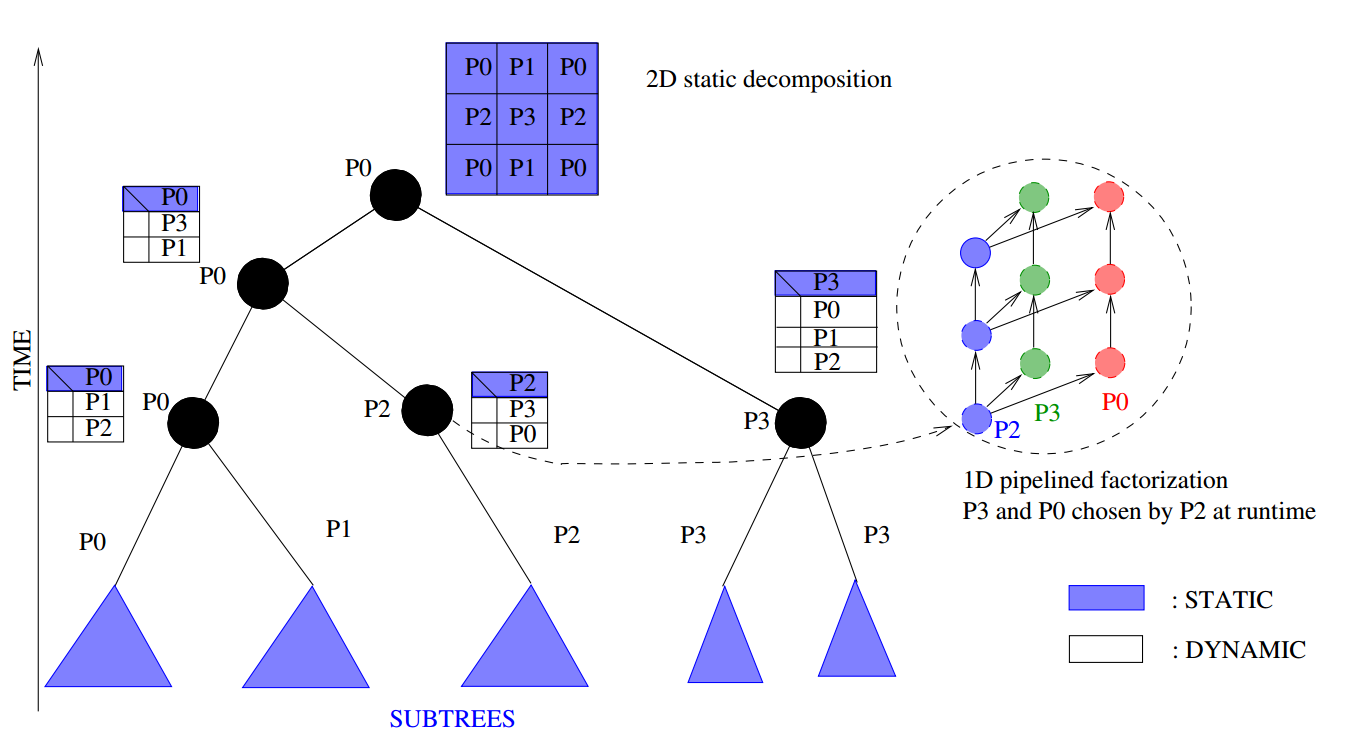
\includegraphics[width=0.85\textwidth]{figures/chapter-2/mumps-task-data-parallelism-2.png}
\caption{MUMPS: static and dynamic scheduling \cite{l2012multifrontal}}
\label{fig:mumps:mapping-and-scheduling}
\end{figure}






%that could measure individual steps of numerical factorization for external packages. During the test we gradually increased the process count and measured the following PETSc parameters: 


%\begin{itemize}

%	\item MatLUFactorSym - time spent on symbolic factorization only (analysis phase)
	
%	\item MatLUFactorNum - time spent on numerical factorization only
	
%	\item PCSetUP - total time spent on $LU$ decomposition including all steps and overheads 
	
%	\item PCApply - time spent on forward and backward substitutions
%\end{itemize}





\section{Choice of BLAS Library}
\label{subseq:blas-comparison}
% Choice of blas labraries




\section{MPI-OpenMP Tuning of MUMPS Library}
\label{subseq:mpi-openmp}


\section{Conclusions}
\label{subseq:conclusions}


% hybrid: we thought it was a hard-ware specific problem, but it turned out it was algoritymic problem!

% additional speed up can be achieved by using faster hardware or better algorithm for time integration




\section{Outlook}
\label{subseq:part-2-outlook}

\begin{itemize}
	\item Optimization engine for preconditioner parameter search.
	% hyperopt, SNOWPAC, Spearmint
	% problems: timeout should be move to the C code in order to estimate error reduction. It can help to determine quality of the preconditioner

	
	\item invasive computing (resource-aware programming)
	% it can help to find an optimal amout of PEs for a running problem
		
	
\end{itemize}